\documentclass[english,11pt,a4paper]{article}
\usepackage[T1]{fontenc} % --------------| More characters.
\usepackage[utf8]{inputenc} % ---------| Direct use of scandinavian letters.
\usepackage{float} % --------------------| More options for floats.
\usepackage{graphicx} % -----------------| Support more image formats.
\usepackage{booktabs} % -----------------| Better-looking tables.
\usepackage{tabularx} % -----------------| Better tables
\usepackage{subfig} % -------------------| Subfigures.
\usepackage[a4paper]{geometry} % --------| Adjusting page margins.
\usepackage{amsmath,amssymb,amsfonts} % -| Various math, including eqref.
\usepackage{xcolor} % --------------------| Allows defn. of custom colors.
\usepackage{babel}
\usepackage{url}

% XY-pic. Used for creating illustrations.
\input xy
\xyoption{all}

% Styling captions.
\usepackage{caption}
\captionsetup{margin=10pt,font=small,labelfont=bf}


%******************************************************************************
% This preabmle contains packages needed to create figures and plots in LaTeX.
%******************************************************************************

\usepackage{etex}
\usepackage{tikz,pgfplots}
\pgfplotsset{compat=1.9}
\usetikzlibrary{calc}
\usetikzlibrary{fit}
\usetikzlibrary{shapes,snakes}
\usetikzlibrary{arrows,decorations.markings}

% Vector Styles for drawings
\tikzstyle{load}   = [ultra thick,-latex]
\tikzstyle{stress} = [-latex]
\tikzstyle{dim}    = [latex-latex]
\tikzstyle{axis}   = [-latex,black!55]


\tikzset{three sided bottom/.style={
        draw=none,
        append after command={
            [shorten <= -0.5\pgflinewidth]
            ([shift={(-1.5\pgflinewidth,-0.5\pgflinewidth)}]\tikzlastnode.north east) % North edge
        edge([shift={( 0.5\pgflinewidth,-0.5\pgflinewidth)}]\tikzlastnode.north west) % North edge
            ([shift={(-0.5\pgflinewidth,-0.5\pgflinewidth)}]\tikzlastnode.north east) % East edge
        edge([shift={(-0.5\pgflinewidth,-0.0\pgflinewidth)}]\tikzlastnode.south east) % East edge
            ([shift={( 0.5\pgflinewidth,-0.5\pgflinewidth)}]\tikzlastnode.north west) % West edge
        edge([shift={( 0.5\pgflinewidth,+0.5\pgflinewidth)}]\tikzlastnode.south west) % West edge
            % ([shift={( 0.5\pgflinewidth,+0.5\pgflinewidth)}]\tikzlastnode.south west) % South edge
        % edge([shift={(-1.0\pgflinewidth,+0.5\pgflinewidth)}]\tikzlastnode.south east) % South edge

        }
    }
}

\tikzset{three sided top/.style={
        draw=none,
        append after command={
            [shorten <= -0.5\pgflinewidth]
            % ([shift={(-1.5\pgflinewidth,-0.5\pgflinewidth)}]\tikzlastnode.north east) % North edge
        % edge([shift={( 0.5\pgflinewidth,-0.5\pgflinewidth)}]\tikzlastnode.north west) % North edge
            ([shift={(-0.5\pgflinewidth,-0.5\pgflinewidth)}]\tikzlastnode.north east) % East edge
        edge([shift={(-0.5\pgflinewidth,-0.0\pgflinewidth)}]\tikzlastnode.south east) % East edge
            ([shift={( 0.5\pgflinewidth,-0.5\pgflinewidth)}]\tikzlastnode.north west) % West edge
        edge([shift={( 0.5\pgflinewidth,+0.5\pgflinewidth)}]\tikzlastnode.south west) % West edge
            ([shift={( 0.5\pgflinewidth,+0.5\pgflinewidth)}]\tikzlastnode.south west) % South edge
        edge([shift={(-1.0\pgflinewidth,+0.5\pgflinewidth)}]\tikzlastnode.south east) % South edge

        }
    }
}

\tikzset{rectangle split h/.style={
    draw, rectangle split, rectangle split parts=#1, rectangle split horizontal
}}


\tikzset{underbrace/.style={
    thick,
    decoration={
        brace,
        mirror,
    },
    decorate
}}

\tikzset{overbrace/.style={
    thick,
    decoration={
        brace,
    },
    decorate
}}

\tikzset{overbrace label/.style={
    pos=0.5,anchor=south,yshift=0.2cm
}}

\tikzset{underbrace label/.style={
    pos=0.5,anchor=north,yshift=-0.2cm
}}

%******************************************************************************
% Custom environment definitions.
% REQUIRES the `color' package.
%******************************************************************************

\usepackage[amsmath,thmmarks,framed]{ntheorem} % Used to define environments
\usepackage{framed} % -------------------------| Used for framed environments
\usepackage{pstricks} % -----------------------| Used for shaded environments
\definecolor{env-gray}{rgb}{0.9,0.9,0.9}

% Examples environment
\theoremstyle{break}
\theoremframepreskip{1em}
\theoremframepostskip{1.5em}
\theoreminframepreskip{0.8em}
\theoreminframepostskip{0.8em}
\newframedtheorem{example}{\protect\examplename}[section]

% Remarks environment
\theoremstyle{plain}
\theorempreskip{1.5em}
\theorempostskip{1.5em}
\newtheorem{remark}{\protect\remarkname}[section]

% Definitions environment
\theoremstyle{plain}
\theoremframepreskip{\topsep}
\theoremframepostskip{\topsep}
\theoreminframepreskip{0.8em}
\theoreminframepostskip{0.8em}
\theoremindent=1em
\theoremrightindent=1em
\def\theoremframecommand{\colorbox{env-gray}}
\newshadedtheorem{definition}{\protect\definitionname}

% Question environment
\theoremstyle{nonumberbreak}
\theoremframepreskip{\topsep}
\theoremframepostskip{\topsep}
\theoreminframepreskip{0.8em}
\theoreminframepostskip{0.8em}
\theoremindent=1em
\theoremrightindent=1em
\def\theoremframecommand{\colorbox{env-gray}}
\newshadedtheorem{question}{\protect\questionname}

% Program output environment
\theoremstyle{nonumberbreak}
\theoremframepreskip{\topsep}
\theoremframepostskip{\topsep}
\theoreminframepreskip{0.8em}
\theoreminframepostskip{0.8em}
\theoremindent=1em
\theoremrightindent=1em
\def\theoremframecommand{\colorbox{env-gray}}
\newshadedtheorem{programoutput}{\protect\programoutputname}


%---------------------------------
% Translations
%---------------------------------
\addto\captionsenglish{\renewcommand{\corollaryname}{Corollary}}
\addto\captionsenglish{\renewcommand{\definitionname}{Definition}}
\addto\captionsenglish{\renewcommand{\examplename}{Example}}
\addto\captionsenglish{\renewcommand{\remarkname}{Remark}}
\addto\captionsenglish{\renewcommand{\questionname}{Question}}
\addto\captionsenglish{\renewcommand{\programoutputname}{Output}}
\addto\captionsnorsk{\renewcommand{\corollaryname}{Korollar}}
\addto\captionsnorsk{\renewcommand{\definitionname}{Definisjon}}
\addto\captionsnorsk{\renewcommand{\examplename}{Eksempel}}
\addto\captionsnorsk{\renewcommand{\remarkname}{Merknad}}
\addto\captionsnorsk{\renewcommand{\questionname}{Spørsmål}}
\addto\captionsnorsk{\renewcommand{\programoutputname}{Output}}
\providecommand{\corollaryname}{Korollar}
\providecommand{\definitionname}{Definisjon}
\providecommand{\examplename}{Eksempel}
\providecommand{\remarkname}{Merknad}
\providecommand{\questionname}{Spørsmål}
\providecommand{\programoutputname}{Output}

%******************************************************************************
% Includes the listings package and sets some settings for it.
% REQUIRES the `color' package.
%******************************************************************************

\usepackage{listings} % -----------------------| Used for source code listings.
\definecolor{lst-gray}{RGB}{100,100,100}  % ---|Color for line-numbers.
\definecolor{lst-light-gray}{RGB}{250,250,250} % Background color for listings.
\definecolor{lst-dark-green}{RGB}{45,111,0} % -| Dark green for comments.
\lstset{
  aboveskip=0em, % -------------------| Skip above listing box.
  backgroundcolor=\color{lst-light-gray}, % Background color.
  basicstyle=\ttfamily\scriptsize, % -| Default font style.
  belowskip=\topskip, % --------------| Skip below listing box.
  breakatwhitespace=false, % ---------| Automatic breaks only at whitespace?.
  breaklines=true, % -----------------| Sets automatic line breaking.
  captionpos=t, % --------------------| Sets the caption-position to bottom.
  commentstyle=\color{lst-dark-green}, % ------| Comment style.
  escapeinside={\%*}{*)}, % ----------| For adding LaTeX within code.
  frame=single, % --------------------| Adds a frame around the code.
  keepspaces=true, % -----------------| Keeps spaces in text.
  keywordstyle=\color{blue}, %--------| Keyword style.
  language={C}, % --------------------| The language of the code.
  literate={æ}{{\ae}}1 % -------------| Character conversions
           {Æ}{{\AE}}1
           {ø}{{\oe}}1
           {Ø}{{\OE}}1
           {å}{{\aa}}1
           {Å}{{\AA}}1
           {µ}{{\ensuremath{\mu}}}1,
  numbers=left, % --------------------| Line-number position: none/left/right.
  numbersep=5pt, % -------------------| Distance between line-numbers and code.
  numberstyle=\tiny\color{lst-gray}, %| The style that used for line-numbers.
  rulecolor=\color{black}, % ---------| Frame color.
  showspaces=false, % ----------------| Show spaces with underscores.
  showstringspaces=false, % ----------| Underline spaces within strings.
  showtabs=false, % ------------------| Show tabs with underscores.
  stepnumber=1, %---------------------| Step between two line-numbers..
  stringstyle=\color{red}, % ---------| String literal style.
  tabsize=4, % -----------------------| Sets default tabsize to 2 spaces.
  title=\lstname % -------------------| Show the filename of included file.
}

\begin{document}

\begin{titlepage}
    \author{Einar Baumann}
    \title{Introduction to Supercomputers: Notes}
    \date{\today}
    \maketitle
\end{titlepage}

\tableofcontents \clearpage

\numberwithin{equation}{section}
\numberwithin{figure}{section}

% -*- root: ../supcom.tex -*-

\section{Symbols} % (fold)
\label{sec:symbols}

\begin{center}
  \begin{tabular}{p{2cm}p{12cm}}
    \toprule
    $\tau_A, \tau_F$ & Time to do a flop, typicall 1/clock frequency. \\
    $\tau_C$         & Linear time to send $b$ bytes. \\
    $\tau_S$         & Latency; time for the first number to arrive (startup time). \\
    $\gamma$         & Inverse bandwidth; time it takes to send one unit of data after the startup time. \\
    \bottomrule
  \end{tabular}
\end{center}

% section symbols (end)
 \clearpage
% -*- root: ../supcom.tex -*-

\section{Timings} % (fold)
\label{sec:timings}

Inner product $\mathbf{x}^T \mathbf{y}$: $n-1$ additions and $n$ multiplications.
\begin{equation}
  T_{ip} = (n-1) + n \approx 2n
\end{equation}

Matrix-vector multiplication $\mathbf{Ax}$, square matrix: ($n-1$) additions and $n$ multiplications for each of $n$ rows:
\begin{equation}
  T_{m\times v} = n((n-1)+n) \approx 2n^2
\end{equation}

Matrix-matrix multiplication $\mathbf{AB}$, sqare matrices: Basically multiplying two $n\times n$ matrices requires performing $n^2$ inner products:
\begin{equation}
  T_{m\times v} = n^((n-1) + n) \approx 2n^3
\end{equation}

% section timings (end)
 \clearpage
% -*- root: ../supcom.tex -*-

\section{Equations} % (fold)
\label{sec:equations}

\subsection{Important equations} % (fold)
\label{sub:important_equations}
Speedup:
\begin{equation}
  S_p = \frac{T_1}{T_p}
\end{equation}
Parallel efficiency:
\begin{equation}
  \eta_p = \frac{S_p}{p} = \frac{T_1}{pT_p}
\end{equation}
Amdahls law (max speedup):
\begin{equation}
  S(N) = \frac{1}{1-B + \frac{B}{N}}
\end{equation}
where $N$ is the number of processors and $B$ is the fraction of the code that can be parallelized.
% subsection important_equations (end)

\subsection{Speedup} % (fold)
\label{sub:speedup}

We use a simple linear network model where the time to send $b$ bytes is modelled as
\begin{equation}
  T^{comm}(b) = \kappa + \gamma b
\end{equation}
where $\kappa$ is the network latency and $\gamma$ the inverse network bandwidth.

For simplicitly we here consider a single Gauss-Jacobi iteration. If we split the matrix by rowsm assuming equal load on each MPI process, we get the computation and communication times
\begin{equation}
  T_P = \frac{T_1}{P}, \quad T_P^{comm} = \kappa + \gamma N^2
\end{equation}
and speedup
\begin{equation}
  S_P = \frac{T_1}{T_P+T_P^{comm}} = \frac{P}{1+P(\kappa + \gamma 8N^2)}
\end{equation}

If we apply domain decompositioning with strip domains, we get
\begin{equation}
  T_P = \frac{T_1}{P}, T_P^{comm} = 2 (\kappa + \gamma N)
\end{equation}

% subsection speedup (end)

% section equations (end)
 \clearpage
% -*- root: ../supcom.tex -*-

\section{Approaches to parallellization} % (fold)
\label{sec:approaches_to_parallellization}

The two approaches to parallellizing a program duscussed in the course are are \emph{Shared Memory} and \emph{Distributed Memory}.

% NUMA utilizes both
% SMP utilizes shared memory


% section approaches_to_parallellization (end)
 \clearpage
% -*- root: ../supcom.tex -*-

\section{Programming models} % (fold)
\label{sec:programming_models}
A node (with 16 physical processors) on Vilje represents a shared memory system where the aggregate memory for the node is globally available to all the 16 processors. A shared memory programming model (i.e., OpenMP) can therefore be used within a single node.

If we want to develop programs which can run on more than one node, we need to use message-passing (i.e., MPI). Even though each node represents a shared memory system, the message-passing programming model may still be used within a node. However, the opposite is not true: a shared programming model cannot be used on a ``pure'' distributed memory system (e.g., on a PC cluster).

Note that a system like vilje, which represents a shared memory system within a node, and a distributed memory system across the nodes, can also be programmed using both programming models within a single program.

\subsection{MPI} % (fold)
\label{sub:mpi}
Message-passing is fundamentally processor-to-processor communication. Only a local, unique memory is directly available to each processor. Both local and remote processes must cooperate in order to exchange data and/or synchronize.

Note that message-passing is a good way to use distributed shared memory machines (ccNUMA) because it provides a way to express memory/data locality.

Some of the key advantages of the message-passing model are:
\begin{description}
  \item[Portability:]  The model can be used on a collection of homogeneous or heterogeneous processors connected by a fast or a slow communication network.
  \item[Performance:] The approach exploits data locality, as well as the availability of a large, aggregate memory.
  \item[Expressiveness:] A limited communication library suffices for most applications.
\end{description}

\begin{figure}[H]
  \centering
  \includegraphics[]{illustrations/programming_models/mpi.pdf}
  \caption{An illustration of the MPI programming model. We have several independent processes, and each of these processes have their own separate program flow.}
  \label{fig:mpi}
\end{figure}

\begin{figure}[H]
  \centering
  \includegraphics[]{illustrations/programming_models/mpi_message.pdf}
  \caption{Illustration of the message passing model. A number of processes are coupled together via a communication network. Each process has a local and unique memory/cache. The processes communicate via explicit message passing. A
message consists of an ``envelope'' which contains sufficient information about whether and when to open the message, as well as information regarding how to interpret the ``body'' of the message (the actual data).}
  \label{fig:message}
\end{figure}

The MPI operations can be classified in four types of operations:
\begin{enumerate}
  \item One-to-one.
  \item One-to-all.
  \item All-to-one.
  \item All-to-all.
\end{enumerate}

One-to-one operations are also referred to as point-to-point operations (send/receive), while the last three types are collective operations. When we say ``all'', we generally mean all processes $P_0, P_1, \dots, P_{n-1}$ in a group of $n$ processes. The default is to let all processes be members of the same default communicator; however they may also be divided into separate groups.

The collective operations may also be broken down into two more categories:
\begin{enumerate}[label=\alph*)]
  \item Data movement: broadcast, gather/scatter.
  \item Collective computation: min/max, sum, etc.
\end{enumerate}

\subsubsection{Six essential functions} % (fold)
\label{ssub:six_essential_functions}
\begin{description}
  \item[\texttt{MPI\_Init}:] Must always be called first (before any other MPI functions).
  \item[\texttt{MPI\_Finalize}:] Ensures a clean exit. Needs to be the last MPI function called.
  \item[\texttt{MPI\_Comm\_size}:] Returns the total number of MPI processes.
  \item[\texttt{MPI\_Comm\_rank}:] Returns the individual process number.
  \item[\texttt{MPI\_Send}:] Send a specified amount of data of a particular data type to a specified process. May also specify a tag.
  \item[\texttt{MPI\_Recv}:] Receive a specified amount of data of a particular data type from a specified process. May also specify a tag. This operation is blocking, and may therefore cause a deadlock.
\end{description}
The syntaxes for MPI\_Send and MPI\_Recv are shown in Figure~\ref{fig:mpi_send_recv}.

\begin{figure}[htbp]
  \centering
  \includegraphics[]{illustrations/programming_models/mpi_send_recv.pdf}
  \caption{The syntaxes for MPI\_Send and MPI\_Recv.}
  \label{fig:mpi_send_recv}
\end{figure}
% subsubsection six_essential_functions (end)



% subsection mpi (end)






\subsection{OpenMP} % (fold)
\label{sub:openmp}
OpenMP is a C/Fortran language extension for programming shared memory parallel machines. It is much more easily implemented than the distributed memory model (MPI), but also poses challenges associated with sharing resources in multiple threads.

It is built on the threading paradigm, combined with a parallel section view of the code. This means that the main program flow happens on \emph{one} processor only. The parallelization is based on a fork/join programming model, as illustrated in Figure~\ref{fig:openmp}.

\begin{figure}[htbp]
  \centering
  \includegraphics[]{illustrations/programming_models/openmp.pdf}
  \caption{An illustration of the OpenMP programming model. We only have a single process, hence the main program flow only happens on a single processor. In sections of the code that we have marked as parallel, the program forks into multiple threads which work independently. At the end of the parallel section, these threads join together again and the program flow is returned to the first processor.}
  \label{fig:openmp}
\end{figure}

In MPI each process has its own private resources. With OpenMP, however, all threads have access to the \emph{same} resources; this is crucial to keep in mind when designating the parallel sections of the code, as the threads might be trying to write to the same memory location (buffer).

\subsubsection{Critical sections} % (fold)
\label{ssub:critical_sections}
If for some reason we need the threads to be able to write to the same resources, this may be achieved by constructing a \emph{critical section} in the code. This lets threads requests locks of a mutex (mutual exclusion lock). When a thread has locked a section of the memory, it is unavailable to all other threads, making them wait for access. This implies a serialization of the program flow over the critical section, which is very bad for the parallel performance.
% subsubsection critical_sections (end)

\subsubsection{Operations suitable for OpenMP parallellization} % (fold)
\label{ssub:operations_suitable_for_openmp_parallellization}
Moderately large computation intensive operations are suitable for OpenMP parallellization. Since thread-dispatchment always has some costs attached, spawning multiple threads easily costs more time than what you gain by doing the calculations in parallel if the operations are too small.

The computations must also be decoupled, since the threads are sharing resources.
% subsubsection operations_suitable_for_openmp_parallellization (end)

\subsubsection{Using OpenMP} % (fold)
\label{ssub:using_openmp}
The idea behind OpenMP is that we give the compiler instructions on which sections of code we want to be parallelized. This means that (unlike MPI) OpenMP requires specific support in the compiler. The compiler then handles the work division between the available number of threads. Note that these instructions are \emph{not} part of the programming language itself, in contrast to MPI.

The instructions given to the compiler are known as \emph{pragma} commands. There are mainly two classes of OpenMP pragmas:
\begin{enumerate}
  \item Pragmas used in combination with loop constructs.
  \item Pragmas used to specify sections of the code which are completely independent of each other.
\end{enumerate}

To parallelize a \texttt{for}-loop in C, we simply add one pragma command:
\begin{lstlisting}
#pragma omp parallel for schedule(static)
for (int i=0; i<100; ++i)
  DoSomething(i);
\end{lstlisting}
Here we are assuming that does not depend on any global resources, and that \texttt{DoSomething(i)} has a constant cost. The pragma can be broken down into three parts:
\begin{description}
  \item[\texttt{\#pragma omp}] All OpenMP directives start with this.
  \item[\texttt{parallel for}] Instructs the compiler that we want the following \texttt{for} construct to be parallelized.
  \item[\texttt{schedule static}] Instructs he compiler to hand each thread approximately the same number of loop iterations up front. This is a good solution here since (we have assumed that) each call to DoSomething(i) has the same cost. Hence such a simple division will give good load balancing between the threads.
\end{description}

In cases where each call to \texttt{DoSomething(i)} has a different cost we may end up with a poor load balancing between the threads (some threads be finish long before others). OpenMP has a mechanism to handle these situations: we simply use a different schedule parameter. We can for example do
\begin{lstlisting}
#pragma omp parallel for schedule(dynamic)
for (int i=0; i<100; ++i)
  DoSomething(i);
\end{lstlisting}
This instructs the compiler to use a dynamic workload division. One thread is then reserved as a bookkeeper/negotiator. Within this parallel section this thread has a simple task: keep track of which loop iterations have been performed and hand out a new one to a thread when it requests it.

Note that this works well if \texttt{DoSomething} is fairly costly, but not if it is cheap. If it is cheap, the process of waiting for/handing out iterations may become dominating. We can overcome this by passing a second parameter to the scheduler: \texttt{schedule(dynamic, N)}, where \texttt{N} is the \emph{chunk size}, i.e. the maximum, number of loop iterations that will be handed out at a time. E.g. if \texttt{N=5}, 5 iterations will be handed out to each thread at a time.

A third scheduling variant is \texttt{guided}. This is a variant of the \texttt{dynamic} scheduler where we start out with large chunk sizes. The chunk sizes are then exponentially decreased until we reach a minimum, as specified in the chunk size. The idea here is that allocating large chunks initially is good for performance, since these will typically overlap fairly well. However, when the number of loop iterations left is small, we may end up in a situation where all the remaining loop iterations are allocated to a single thread. This is bad for performance since the other threads would then be left idle. By using progressively smaller chunks, the chance of this happening is reduced.

The second class of OpenMP directives is used to specify sections of the code which are completely independent of each other. If we for example have three functions which are independent of each other we can do
\begin{lstlisting}
#pragma omp parallel sections
{
  #pragma omp parallel section
  {
    DoJob1();
  }
  #pragma omp parallel section
  {
    DoJob2();
  }
  #pragma omp parallel section
  {
    DoJob2();
  }
}
\end{lstlisting}
Each section will then be performed in its own separate thread, before the program flow returns to procesor 0 once all sections have been completed.
% subsubsection using_openmp (end)

\subsubsection{Conclusions} % (fold)
\label{ssub:conclusions}
\begin{itemize}
  \item OpenMP offers easy exploitation of computing resources on shared memory machines. The parallel code is very close to the serial code - it usually only differs by some pragma's which you can tell a compiler to ignore.
  \item The fork-join programming model often is harder to grasp than the distributed model, in particular if several threads need to access the same resources.
  \item Best results are usually achieved if you combine OpenMP and MPI. This is also the model that maps the best to modern hardware, where you typically have a few handfuls of cpu's sharing memory, while using more than that requires a distributed memory programming model.
\end{itemize}
% subsubsection conclusions (end)
% subsection openmp (end)


% section programming_models (end)
 \clearpage
% -*- root: ../supcom.tex -*-

\section{Parallel I/O with MPI-I/O} % (fold)
\label{sec:parallel_i_o_with_mpi_i_o}
HDDs are normally used as secondary storages. Because HDDs only have a single head, it can only perform a single read/write operation at a time. This means that even though multiple processes can initiate reads concurrently, they will be performed in serial, as shown in Figure~\ref{fig:io_serial}. This can transform CPU bound problems to I/O bound problems.  We can improve the read performance by storing our data across multiple HDDs, as shown in Figure~\ref{fig:io_parallel}.

When it comes to output from parallel processes there are several different approaches. A description of two approaches involving serialization follows.
\begin{description}
  \item[Post-mortem assembly:] Each process dumps its data to a separate file, and then custom tailored code is used to read the data into the next application in the computational chain (e.g. visualization). This approach requires doing significantly more I/O operations than necessary, and large parts of it needs to be done in serial.
  \item[Serializing the I/O:] One process is given the responsibility of writing the data to disk. The other processes send their data to this process in a sequential manner. With this approach all output is written serially.
\end{description}


\begin{figure}[htbp]
  \centering
  \includegraphics[]{illustrations/io/serial_file.pdf}
  \includegraphics[]{illustrations/io/serial_file_graph.pdf}
  \caption{Illustration of serial I/O where multiple processes read from a single file.}
  \label{fig:io_serial}
\end{figure}

\begin{figure}[htbp]
  \centering
  \includegraphics[]{illustrations/io/parallel_file.pdf}
  \includegraphics[]{illustrations/io/parallel_file_graph.pdf}
  \caption{Illustration of parallel I/O where we harness the aggregated bandwidth of several devices. Each process reads its data from a separate physical device, enabling parallel I/O.}
  \label{fig:io_parallel}
\end{figure}

\subsection{MPI-IO} % (fold)
\label{sub:mpi_io}
The MPI-IO interface allows us to split the output across multiple storage devices. It needs to be tuned to the underlying filesystem to achieve good performance; one such file system is GPFS (General Parallel FileSystem). Informing the system about the underlying distributed nature of an I/O call enables the system to make good choices about how the I/O is performed on a lower level.
% subsection mpi_io (end)


\subsubsection{Non-sequential I/O: Fileviews} % (fold)
\label{ssub:non_sequential_i_o_fileviews}
We now consider a vector split in a cyclic manner, as shown in Figure~\ref{fig:nonseqio}. We assume that each block consists of a small amount of data; for simplicity a single \texttt{double}. This means that, for each separate process, the data access pattern consists of a single number followed by a gap of $size-1$ numbers.

\begin{figure}[H]
  \centering
  \includegraphics[]{illustrations/io/nonseqio.pdf}
  \caption{Illustration of cyclic file writing. The $P_0$ block is written by $P_0$ etc.}
  \label{fig:nonseqio}
\end{figure}


MPI has a builtin machinere to describe custom datatypes. These were originally intended to be used to describe data layout in memory, but they can also be used to describe data patterns on secondary storage. This datatype is constructed as follows:
\begin{lstlisting}
MPI_Datatype filetype;
MPI_Type_create_resized(MPI_DOUBLE,          // Old type
                        0,                   // Lower bound
                        size*sizeof(double), // Extent
                        &filetype            // Output datatype
                        );
MPI_Type_commit(&filetype);
\end{lstlisting}

We then attach this datatype as a process' \emph{view} into the file using the function
\begin{lstlisting}
MPI_File_set_view(fh,                  // File handle
                  rank*sizeof(double), // Displacement from beginning of file,
                  MPI_DOUBLE,          // Elementary data type
                  filetype             // File data type (created above)
                  'native',            // Data representation
                  MPI_INFO_NULL        // Info structure (for tuning)
                  );
\end{lstlisting}

The data is then written to secondary storage using a normal write call on each process:
\begin{lstlisting}
MPI_File_write(fh,               // File handle (with custom view now set)
               vec,              // Buffer to be written
               mysize,           // Number of elements to write (for this process)
               MPI_DOUBLE,       // Datatype of each element
               MPI_STATUS_IGNORE
               );
\end{lstlisting}

The system takes care of inserting the gaps. Since it knows the data access patterns on each process up front, it can optimize how storing the data to disk is perfomed, with large writes and minimal seeks.
% subsubsection non_sequential_i_o_fileviews (end)

\subsubsection{Distributed arrays} % (fold)
\label{ssub:distributed_arrays}
In HPC applications the data is usually consists of matrices or 3D arrays; MPI containts machinery to partition such arrays in semi-automatic ways, and we can benefit from this when we want to write the data to secondary storage.

There are essentially two ways to split an array across processes; these are shown in Figure~\ref{fig:splitting}. The MPI machinery allows us to handle both with essentially the same code. MPI calls such arrays \texttt{darrays} -- distributed arrays. An array partitioning consists of a topology (``descrition of how stuff is connected'') and a mapping of pocesses onto this topology.

\begin{figure}[htbp]
  \centering
  \includegraphics[]{illustrations/io/splitting.pdf}
  \caption{Illustration of the two primary ways to partition a 2D matrix.}
  \label{fig:splitting}
\end{figure}
% subsubsection distributed_arrays (end)

Figure~\ref{fig:topology} contains all the pieces of information we need to descirbe a topology and mapping:
\begin{itemize}
  \item A global cartesian topology, expressed as the number of processes along each dimension (2,3).
  \item Location of a particular domain in the topology; again this can be expressed as an integer along each dimension.
  \item A mapping of the available processes onto the topology.
\end{itemize}

\begin{figure}[htbp]
  \centering
  \includegraphics[]{illustrations/io/topology.pdf}
  \caption{``Schematic'' of a topology mapping.}
  \label{fig:topology}
\end{figure}

To realize this in MPI, we first generate a cartesian partitioning using \texttt{MPI\_Dims\_create}:
\begin{lstlisting}
int sizes = [2];
sizes[0] = sizes[1] = 0;
MPI_Dims_create(size, // Number of nodes in the grid
                2,    // Number of cartesian dimensions
                sizes // IN: Dims to partition over; OUT: Nodes in each dimension
                );
\end{lstlisting}
The function only operates over dimensions where $sizes=0$, so if we instead wanted a strip partitioning we could just change the code to \texttt{sizes[0]=1}. On return, the \texttt{sizes} arrays contains the partitioning in each dimension.

In order to be able to generate the mapping of processes onto the topology, we need to define a communicator which has the topology attached.
\begin{lstlisting}
int periodic[2];
periodic[0] = periodic[1] = 0; // NOT periodic in both dimensions
MPI_Comm comm;
MPI_Cart_create(MPI_COMM_WORLD, // Input communicator
                2,              // Number of cartesian dimensions
                sizes,          // Number of processes in each dimension
                periodic,       // Periodic (or not) in each dimension
                0,              // Reordered (or not). Here not.
                &comm           // Output communicator
                );
\end{lstlisting}
Upon return the \texttt{comm} variable holds the new communicator.

The individual processes can now query where they are placed in the topology using the function:
\begin{lstlisting}
int coords[2];
MPI_Cart_coords(comm, // Communicator
                rank, // Rank of process
                2,    // Max dims (length of coords)
                coords // OUT: Coordinates in grid
                );
\end{lstlisting}
On process 5 this would return a \texttt{coords} array containing 1 and 2.

We can now use the \texttt{MPI\_Type\_create\_darray} function to generate the datatype and file view on each process:
\begin{lstlisting}
MPI_Type_create_darray(size,     // Size of process group
                       rank,     // Rank in process group
                       dims,     // #array dimensions/process grid dimensions
                       gsizes,   // #elements of old type in each dim (global)
                       distribs, // Distribution strategies in each dimesnsion
                       dargs,    // Distribution strategy
                       sizes,    // Size of process grid in each dimension
                       order,    // Array layout in memory
                       etype,    // Type of array entries
                       newtype   // New type (OUT)
                       );
MPI_Type_commit(&newtype);
\end{lstlisting}

\subsubsection{Non-blocking I/O -- Overlapping I/O and computations} % (fold)
\label{ssub:non_blocking_i_o_overlapping_i_o_and_computations}
On modern architectures HDDs can write/read data completely on their own using a technique known as \emph{Direct Memory Access}. Likewise, network components can do the same (if the HDDs are not locally attached). This means that while we are reading/writing data, the CPU is mostly an idle observer. This is bad for program efficiency - we want to keep the CPUs saturated with work.

MPI offers facilities to remedy this, namely non-blocking I/O operations.

% TODO

% subsubsection non_blocking_i_o_overlapping_i_o_and_computations (end)




% section parallel_i_o_with_mpi_i_o (end)
 \clearpage
% -*- root: ../supcom.tex -*-

\section{Pipelining} % (fold)
\label{sec:pipelining}


Lets say we want to add the three vectors $\vec{a}, \vec{b}$ of lenght $n$ and store the result in vector $\vec{c}$:
\begin{equation}
  \vec{c} = \vec{a} + \vec{b}
\end{equation}

Normally, each of the $n$ additions takes five clock cycles:
\begin{enumerate}
  \item Read from register.
  \item Align.
  \item Add.
  \item Pack.
  \item Write to register.
\end{enumerate}
which means that we could expect that the total number of clock cycles required for the operation is $5n$ and that the total execution time is $5n\tau$. However, by using pipelining, we can get this down to $n\tau$ for $n\gg 1$. This is because pipelining lets us start reading the next pair of numbers from the register while we're aligning the previous two, etc. After a startup time, we will then get one value $c(i)$ pr. clock cycle.
% section pipelining (end)

\subsection{Superscalar operations} % (fold)
\label{sub:superscalar_operations}
Superscalar operations means that two operations are chained together in a pipeline; e.g. multiply and add as shown in Figure~\ref{fig:superscalar}. This works in approximately the same way as pipelining in general; but we will after a slightly longer time get two floating point operations pr. clock cycle (theoretically).


\begin{figure}[htbp]
  \centering
  \includegraphics[]{illustrations/processor/superscalar.pdf}
  \caption{The superscalar operation multiply and add.}
  \label{fig:superscalar}
\end{figure}

% subsection superscalar_operations (end)
 \clearpage
% -*- root: ../supcom.tex -*-

\section{Cache} % (fold)
\label{sec:cache}

The main purpose of the cache is to keep copies of data in extra (fast) memory close to the CPU in order to ``hide'' the relatively slow transfer rate between the main memory and the processor.

The cahce is smaller than the main memory by some power of two. Hence, a strategy for mapping memory locations to the cache is needed. One such strategy is direct mapping.

\subsection{Direct mapping} % (fold)
\label{sub:direct_mapping}

With the direct mapping strategy, illustrated in Figure~\ref{fig:direct}, each location in main memory corresponds to a unique location in cache. Because only the first bits of the main memory address are used when we're mapping the blocks to cahce (Figure~\ref{fig:address}), we see that several main memory addresses map to the same cache address.

\begin{figure}[htbp]
  \centering
  \includegraphics[]{illustrations/cache/direct.pdf}
  \caption{Each location in memory can be mapped to exactly one cahce line.}
  \label{fig:direct}
\end{figure}

\begin{figure}[htbp]
  \centering
  \includegraphics[]{illustrations/cache/memory-address.pdf}
  \caption{The main memory address is split into two parts: the first bits are called the \emph{set bits}, and give the precise cache address. The remaining parts are the \emph{tag bits} and are used to determine if a copy of the content at the particular main memory location has been copied into the cache location given by the set bits.}
  \label{fig:address}
\end{figure}

Note that, when a floating point number (or an integer) is requested by the program, more than a single number is copied into cache. The minimum amount of data copied is called a \emph{cache line}.
% subsection direct_mapping (end)

\subsection{Cache trashing} % (fold)
\label{sub:cache_trashing}
As stated in the above section, several addresses in main memory may map to the same address. This may cause problems if for examble we're adding two vectors $a,b$ to produce the vector $c$, which fill its own block in memory. If these blocks all map to the same cache line (and we're using direct mapping) they can never be in the cahce at the same time. They will need to be brought in from main memory every time, causing a severe drop in performance. This is called \emph{cache trashing}.

Cache trashing may in this case be avoided by storing the vectors in a different manner, i.e.
\begin{equation}
\nonumber
  a(1),b(1),c(1),(a2), (b2), c(2), \dots, a(n), b(n), c(n)
\end{equation}
instead of
\begin{equation}
  \nonumber
  a(1),a(2),\dots,a(n),b(1),b(2),\dots, b(n), c(1), \dots
\end{equation}
% subsection cache_trashing (end)

\subsection{$n$-way set-associative mapping} % (fold)
\label{sub:_n_way_associative_mapping}
An alternative strategy for mapping memory locations is $n$-way set-associative, illustrated in Figure~\ref{fig:cache-n-way}. Here there are $n$ ways to map a memory address to a cache address, i.e. a memory location can potentially end up in one of $n$ cache lines. The particural line chosen depends on the replacement policy:
\begin{itemize}
  \item Least Recently Used (LRU).
  \item Least Frequently Used (LFU).
  \item Random.
\end{itemize}
In the context the algorithms used in this course, LRU gives the best performance. This is because the problems exhibit locality in time and space.

\begin{figure}[htbp]
  \centering
  \includegraphics[]{illustrations/cache/n-way.pdf}
  \caption{An illustration of $n$-way set-associative cache. Each block in memory can map to $n$ different locations in the cache.}
  \label{fig:cache-n-way}
\end{figure}

\begin{figure}[htbp]
  \centering
  \includegraphics[]{illustrations/cache/set-associative.pdf}
  \caption{Set-associative mapping. The set part gives the set (1/2/3) the data is in; the tag gives the line within the set; the offset gives the location on the line.}
  \label{fig:set-associative}
\end{figure}

\begin{figure}[htbp]
  \centering
  \includegraphics[]{illustrations/cache/2-way.pdf}
  \caption{2-way cache mapping. Each memory location can map to two different cache lines.}
  \label{fig:label}
\end{figure}
% subsection _n_way_associative_mapping (end)



% section cache (end)
 \clearpage
% -*- root: ../supcom.tex -*-

\section{Solving the Poisson equation} % (fold)
\label{sec:solution_methods}

\subsection{Cholesky factorization} % (fold)
\label{sub:banded_cholesky}

If the matrix $\mathbf{A}$ is symmetric and positive definite, we find that $\mathbf{U}=\mathbf{L}^T$. Thus we can save a factor 2 in memoy and a factor 2 in required FLOP. Furthermore, no pivoting is required for such systems. This is called a \emph{Cholesky factorization}.

% subsection banded_cholesky (end)


\subsection{Krylov subspace methods} % (fold)
\label{sub:krylov_subspace_methods}
For any vector $b$,
\begin{equation}
  \mathbf{x} = \sum_{j=0}^{N-1} v_j \mathbf{A}^j \mathbf{b}
\end{equation}
that is span $\left\{ \mathbf{A}^j \mathbf{b} \right\}_{j=0}^{N-1}$ form a basis for the column space of $\mathbf{A}$. We call this space the \emph{Krylov subspace} of $\mathbf{A}$. Here $v_j$ is a set of coefficients. The main idea behind the Krylov subspace methods is to make an initial guess, then improve this by successively  eliminating contributions to the residual akibg each Krylov vector.

Many different Krylov methods exist, each suitable for different types of linear systems (in the sense of symmetries, dfiniteness etc.).

\subsubsection{Conjugate gradient (CG)} % (fold)
\label{ssub:conjugate_gradient}

The \emph{conjugate gradient} method is one of the two most important Krylov methods. The algorithm for the CG method is as follows:

\begin{algorithm}[H]
  \SetKwInput{KwSet}{Set}
  \KwSet{$\mathbf{u}^0=\mathbf{0}, \mathbf{r}^0=\mathbf{f}$}
  \For{$m=1,2,...$}{
    $\beta_{m}=\frac{\left(\mathbf{r}^{m-1}\right)^{T}\mathbf{r}^{m-1}}{\left(\mathbf{r}^{m-2}\right)^{T}\boldsymbol{r}^{m-2}}\qquad\qquad(\beta_{1}\equiv0)$ \;
    $\boldsymbol{p}^{m}=\boldsymbol{r}^{m-1}+\beta_{m}\boldsymbol{p}^{m-1}\qquad(\boldsymbol{p}^{1}\equiv\boldsymbol{r}^{0})$ \;
    $\alpha_{m}=\frac{\left(\boldsymbol{r}^{m-1}\right)^{T}\boldsymbol{r}^{m-1}}{\left(\boldsymbol{p}^{m}\right)^{T}\boldsymbol{A}\boldsymbol{p}^{m}}$ \;
    $\boldsymbol{u}^{m}=\boldsymbol{u}^{m-1}+\alpha_{m}\boldsymbol{p}^{m}$ \;
    $\boldsymbol{r}^{m}=\boldsymbol{r}^{m-1}-\alpha_{m}\boldsymbol{A}\boldsymbol{p}^{m}$ \;
  }
  \caption{The conjugate gradient method.}
\end{algorithm}

Both this method and the GMRES method in the next section are hybrid method; part direct, part iterative. If we eliminate along all Krylov vectors we get the exact solution (if done with exact arithmetics). However, we use it as a way to obtain an approximative solution by introducing a stopping criterion. A typical cirterion is $\vert\vert r \vert\vert < tol$ for some tolerance $tol$.






% subsubsection conjugate_gradient (end)







\subsubsection{GMRES: Generalized Minimum RESidual method} % (fold)
\label{ssub:gmres_generalized_minimum_residual_method}
The GMRES is the ``hammer'' among the Krylov methods: it handles non-symmetric and non-definite problems.

% subsubsection gmres_generalized_minimum_residual_method (end)

% subsection krylov_subspace_methods (end)

\subsection{Monte Carlo methods} % (fold)
\label{sub:monte_carlo_methods}
Monte Carlo methods are a broad class of computational algorithms that rely on repeated random sampling to obtain numerical results; typically one runs simulations many times over in order to obtain the distribution of an unknown probabilistic entity. In physics-related problems, Monte Carlo methods are quite useful for simulating systems with many coupled degrees of freedom, such as fluids, disordered materials, strongly coupled solids, and cellular structures.

Monte Carlo methods vary, but tend to follow a particular pattern:
\begin{enumerate}
  \item Define a domain of possible inputs.
  \item Generate inputs randomly from a probability distribution over the domain.
  \item Perform a deterministic computation on the inputs.
  \item Aggregate the results.
\end{enumerate}

For example, consider a circle inscribed in a unit square. Given that the circle and the square have a ratio of areas that is $\pi/4$, the value of $\pi$ can be approximated using a Monte Carlo method:
\begin{enumerate}
  \item Draw a square on the ground, then inscribe a circle within it.
  \item Uniformly scatter some objects of uniform size (grains of rice or sand) over the square.
  \item Count the number of objects inside the circle and the total number of objects.
  \item The ratio of the two counts is an estimate of the ratio of the two areas, which is $\pi/4$. Multiply the result by 4 to estimate $\pi$.
\end{enumerate}
In this procedure the domain of inputs is the square that circumscribes our circle. We generate random inputs by scattering grains over the square then perform a computation on each input (test whether it falls within the circle). Finally, we aggregate the results to obtain our final result.

If the grains are not uniformly distributed, then our approximation will be poor. Secondly, there should be a large number of inputs. The approximation is generally poor if only a few grains are randomly dropped into the whole square. On average, the approximation improves as more grains are dropped.


\subsubsection{Integration by use of Monte Carlo methods} % (fold)
\label{ssub:integration_by_use_of_monte_carlo_methods}
Monte Carlo methods are well suited for use in problems with many degrees of freedom/dimensions. As long as the function in question is reasonably well-behaved, it can be estimated by randomly selecting points in $n$-dimensional space, and taking some kind of average of the function values at these points. By the central limit theorem, this method displays $1/\sqrt{N}$ convergence; i.e. quadrupling the number of sampled points halves the error, regradless of the number of dimensions.
% subsubsection integration_by_use_of_monte_carlo_methods (end)

% subsection monte_carlo_methods (end)

% section solution_methods (end)


\clearpage
\subsection{Poisson matrix formats} % (fold)
\label{sec:poisson_matrix_format}

\subsection{1 dimension} % (fold)
\label{sub:1_dimension}

\[
  \begin{bmatrix}
    2 & -1 & 0 & 0 & 0 & 0 \\
    -1 & 2 & -1 & 0 & 0 & 0 \\
    0 & -1 & 2 & -1 & 0 & 0 \\
    0 & 0 & -1 & 2 & -1 & 0 \\
    0 & 0 & 0 & -1 & 2 & -1 \\
    0 & 0 & 0 & 0 & -1 & 2 \\
  \end{bmatrix}
\]
% subsection 1_dimension (end)

\subsection{2 dimensions} % (fold)
\label{sub:2_dimensions}

\[
  \begin{bmatrix}
    4 & -1 & 0 & \cdots & -1 & 0 & \cdots & \cdots & 0\\
    -1 & 4 & -1 & \ddots & \cdots & -1 & \ddots & \ddots & \vdots\\
    0 & -1 & 4 & -1 & \ddots & \cdots & -1 & \ddots & \vdots\\
    \vdots & \ddots & \ddots & \ddots & \ddots & \ddots & \cdots & \ddots & 0\\
    -1 & 0 & \ddots & -1 & 4 & -1 & \ddots & 0 & -1\\
    0 & \ddots & \ddots & \ddots & \ddots & \ddots & \ddots & \ddots & 0\\
    \vdots & \ddots & \ddots & \ddots & \ddots & \ddots & \ddots & \ddots & \vdots\\
    \vdots & \ddots & \ddots & \ddots & \ddots & \ddots & \ddots & \ddots & -1\\
    0 & \cdots & \cdots & 0 & -1 & \cdots & 0 & -1 & 4
  \end{bmatrix}
\]

% subsection 2_dimensions (end)

% section poisson_matrix_format (end)
 \clearpage
% -*- root: ../supcom.tex -*-

\section{Banded matrices} % (fold)
\label{sec:banded_matrices}

A banded matrix is a sparse matrix whose non-zero entries are confined to a diagonal band, comprising the main diagonal and zero or more diagonals on either side.

\subsection{Matrix bandwidth} % (fold)
\label{sub:matrix_bandwidth}
Formally, consider an $n\times n$ matrix $\mathbf{A}=(a_{i,j})$. If all matrix elements are zero outside a diagonally bordered band whose range is determined by constants $k_1$ and $k_2$:
\[
  a_{i,j} = 0 \; \text{if} \; j < i-k_1 \quad \text{or} \quad j > i + k_2; \quad k_1, k_2 > 0
\]
then the quantities $k_1$ and $k_2$ are called the \emph{left} and \emph{right half-bandwidth}, respectively. The \emph{bandwidth} $b$ of the matrix is
\begin{equation}
  b = k_1+k_2+1
\end{equation}
In other words, it is the smallest number of adjacent diagonals to which to which the non-zero elements are confined.

A matrix is called a \emph{banded matrix} if the bandwidth is reasonably small.

A banded matrix with $k_1=k_2=0$ is a diagonal matrix; a banded matrix with $k_1=k_2=1$ is a tridiagonal matrix; etc. If one puts $k=0, k_2=n-1$ one obtains the definition of an upper triangular matrix; similarly for $k_1=n-1, k_2=0$ one obtains a lower triangular matrix.

The following three matrices are all $n\times n$ matrices with $n=6$. The first one has $k_1=k_2=0$; the second one has $k_1=k_2=1$; the third one has $k_1=0, k_2=n-1$.


\[
  \begin{bmatrix}
    1 & 0 & 0 & 0 & 0 & 0 \\
    0 & 1 & 0 & 0 & 0 & 0 \\
    0 & 0 & 1 & 0 & 0 & 0 \\
    0 & 0 & 0 & 1 & 0 & 0 \\
    0 & 0 & 0 & 0 & 1 & 0 \\
    0 & 0 & 0 & 0 & 0 & 1 \\
  \end{bmatrix}
  \quad
  \begin{bmatrix}
    1 & 1 & 0 & 0 & 0 & 0 \\
    1 & 1 & 1 & 0 & 0 & 0 \\
    0 & 1 & 1 & 1 & 0 & 0 \\
    0 & 0 & 1 & 1 & 1 & 0 \\
    0 & 0 & 0 & 1 & 1 & 1 \\
    0 & 0 & 0 & 0 & 1 & 1 \\
  \end{bmatrix}
  \quad
  \begin{bmatrix}
    1 & 1 & 1 & 1 & 1 & 1 \\
    0 & 1 & 1 & 1 & 1 & 1 \\
    0 & 0 & 1 & 1 & 1 & 1 \\
    0 & 0 & 0 & 1 & 1 & 1 \\
    0 & 0 & 0 & 0 & 1 & 1 \\
    0 & 0 & 0 & 0 & 0 & 1 \\
  \end{bmatrix}
\]
% subsection matrix_bandwidth (end)

\subsection{Band storage} % (fold)
\label{sub:band_storage}

Banded matrices are usually stored by storing the diagonals in the band as columns; the rest is implicity zero. What follows is an example of storing a $6\times 6$ tridiagonal matrix in a $6\times 3$ matrix:
\[
  \begin{bmatrix}
    B_{11} & B_{12} & 0      & \cdots & \cdots & 0      \\
    B_{21} & B_{22} & B_{23} & \ddots & \ddots & \vdots \\
    0      & B_{32} & B_{33} & B_{34} & \ddots & \vdots \\
    \vdots & \ddots & B_{43} & B_{44} & B_{45} & 0      \\
    \vdots & \ddots & \ddots & B_{54} & B_{55} & B_{56} \\
    0      & \cdots & \cdots & 0      & B_{65} & B_{66} \\
  \end{bmatrix}
  \;\rightarrow\;
  \begin{bmatrix}
    0      & B_{11} & B_{12} \\
    B_{21} & B_{22} & B_{23} \\
    B_{32} & B_{33} & B_{34} \\
    B_{43} & B_{44} & B_{45} \\
    B_{54} & B_{55} & B_{56} \\
    B_{65} & B_{66} & 0      \\
  \end{bmatrix}
\]

We can save further space if the matrix is symmetric: we then only have to store the main diagonal plus either the diagonals on the left or the right side. The other side is implicit from what is stored; e.g. $a_{i,i-1}=a_{i,i+1}$.

% subsection band_storage (end)

\subsection{Super- and subdiagonals} % (fold)
\label{sub:super_and_subdiagonals}
A superdiagonal entry is one that is directly above and to the right of the main diagonal. A subdiagonal entry is one that is directly below and to the left of the main diagonal,


% subsection super_and_subdiagonals (end)

% section banded_matrices (end)
 \clearpage
% -*- root: ../supcom.tex -*-

\section{BLAS: Basic Linear Algebra System} % (fold)
\label{sec:blas}

The Basic Linear Algebra Subprograms (BLAS) are a specified set of low-level kernel subroutines that perform common linear algebra operations such as copying, vector scaling, vector dot products, linear combinations, and matrix multiplication.

BLAS operations are divided in three levels
\begin{description}
  \item[Level 1] operations only involve vectors: dot products, vector norms, scaling with a constant, generalized verctor addition (axpy) on the form
    \[
      \mathbf{y} = \alpha \mathbf{x} + \mathbf{y}
    \]
  \item[Level 2] operations are matrix-vector operations, including a generalized matrix vector multiplication (gemv):
    \[
      \mathbf{y} = \alpha \mathbf{A}\mathbf{x} + \beta \mathbf{y}
    \]
  \item[Level 3] operations are matrix-matrix operations includes a general matrix multiplication (gemm):
    \[
      \mathbf{C} = \alpha \mathbf{AB} + \beta \mathbf{C}
    \]
\end{description}

BLAS is column major. This is because it is implemented in FORTRAN, whose notation tries to be consistent with mathematical notation. A C implementation of BLAS -- CBLAS -- also exists. This library can handle row-major matrices.

Note that in general we achieve the highest number of FLOPS with level 3 operations. This is because today computation is generally memory bound; matrix-matrix operations allow for a higher degree of reuse (i.e. more cahce involvement) than the other types (they need to fetch new data from memory at a higher rate). But in general, all computation using BLAS are memory bound today because of high clock frequencies compared to memory speeds.




% section blas (end)
 \clearpage
% -*- root: ../supcom.tex -*-

\section{Matrix-vector multiplication} % (fold)
\label{sec:matrix_multiplication}

This section is based on the notes found at \url{http://www.hpcc.unn.ru/mskurs/ENG/DOC/pp07.pdf}.

\subsection{Problem statement} % (fold)
\label{sub:problem_statement}
The result of multiplying the matrix $A$ of order $m\times n$ by vector $b$, consisting of $n$ elements, is the vector $c$ of size $m$, each $i$-th element of which is the result of the inner multiplication of the $i$-th matrix $A$ row $a_i$ by vector $b$:
\begin{equation}
  c_i = \sum_{j=0}^{n-1} a_{ij}b_j, \quad 0\leq i \leq m-1
\end{equation}

Each operation includes multiplying the matrix row elements by the elements of vector $b$ ($n$ operations) and the following summing the obtained products ($n-l$ operations). The total number of necessary scalar operations is the value
\begin{equation}
  T_1 = m \cdot (2n-1)
\end{equation}
% subsection problem_statement (end)

\subsection{Data distribution} % (fold)
\label{sub:data_distribution}
While executing the parallel algorithm of matrix-vector multiplication, it is necessary to distribute not only the matrix $A$, but also the vector $b$ and the result vector $c$. The vector elements can be duplicated, i.e. all the vector elements can be copied to all the processors of the multiprocessor computer system, or distributed among the processors. In case of block partitioning of the vector consisting of $n$ elements, each processor processes the continuous sequence of $k$ vector elements (we assume that the vector size $n$ is divisible by the number of processors $p$, i.e. $n = k·p$).

Let us make clear, why duplicating vectors $b$ and $c$ among the processors is an admissible decision (for simplicity further we will assume that $m=n$). Vectors $b$ and $c$ consist of $n$ elements, i.e. contain as much data as one matrix row or column. If the processor holds a matrix row or column and single elements of the vectors $b$ and $c$, the total size of used memory is the order $O(n)$. If the processor holds a matrix row (column) and all the elements of the vectors $b$ and $c$, the total number of used memory is the same order $O(n)$. Thus, in cases of vector duplicating and vector distributing the requirements to memory size are equivalent.
% subsection data_distribution (end)

\subsection{Matrix-vector multiplication in case of rowwise data decomposition} % (fold)
\label{sub:matrix_vector_multiplication_in_case_of_rowwise_data_decomposition}
To execute the basic subtask of inner multiplication the processor must contain the corresponding row of matrix $A$ and the copy of vector $b$. After computation completion each basic subtask determines one of the elements of the result vector $c$.

To combine the computation results and to obtain the total vector $c$ on each processor of the computer system, it is necessary to execute the all gather operation, in which each processor transmits its computed element of vector $c$ to all the other processors. This can be executed, for instance, with the use of the function MPI\_Allgather of MPI library.

The general scheme of informational interactions among subtasks in the course of computationS is shown in Figure~\ref{fig:rowwise-scheme}.

\begin{figure}[htbp]
  \centering
  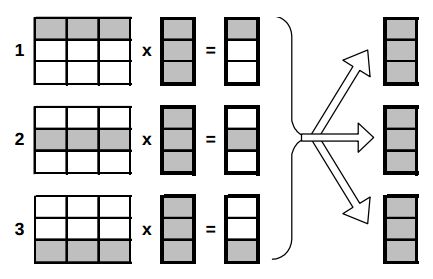
\includegraphics[width=0.5\textwidth]{illustrations/matrix-vector-product/rowwise.png}
  \caption{Computation scheme for parallel matrix-vector multiplication base on rowwise striped matrix partitioning.}
  \label{fig:rowwise-scheme}
\end{figure}


\subsubsection{Efficiency analysis} % (fold)
\label{ssub:efficienct_analysis}
Let us consider the time complexity of the algorithm of matrix-vector multiplication. If matrix $A$ is square $(m=n)$, the sequential algorithm of matix-vector multiplication has the complexity
\begin{equation}
  T_1 = n(n-1+n)\approx 2n^2 = O(n^2)
\end{equation}
In case of parallel computations each processor performs multiplication of only a part (stripe) of the matrix $A$ by the vector $b$. The size of these stripes is equal to $n/p$ rows. In case of computing the inner product of one matrix row by a vector, it is necessary to perform the $n$ multiplications and $(n-l)$ additions. Therefore, computational complexity of the parallel algorithm is determined as:
\begin{equation}
  T_p = \frac{n(n-1+n)}{p} \approx \frac{2n^2}{p} = O(\frac{n^2}{p})
\end{equation}

Taking into accoun this estimation, the criteria of speedup and efficiency of the parallel
\begin{align}
  S_p &= \frac{T_1}{T_p} = \frac{n^2}{n^2/p} = p \\
  E_p &= \frac{T_1}{pT_p} = \frac{n^2}{p(n^2/p)} = 1
\end{align}
These estimations of the computation execution time are expressed in the number of operations. Besides, they are formed \emph{without} taking into consideration the execution of data communication operations. Let us use the above mentioned assumptions that the executed multiplications and additions are of equal duration $\tau_F$.

The computation time of the parallel algorithm is
\begin{equation}
  T_p(calc) = \# rows \times \# ops/row \times \tau_F = \frac{n}{p} \cdot (2n-1) \cdot \tau_F
\end{equation}

After doing the calculations, we use MPI\_Allgather to gather all the $c$-parts on all processors. This works using a binary tree, and so the gather operation can be performed in $\log_2 p$ iterations. In the first iteration, each process sends its part (of size $n/p$) to another process, which in turn will send its own part plus the part it received (total size $2n/p$) on to the next process in the next iteration; thus, the amount of data to be sent doubles in each iteration. As a result, the all gather operation execution time when the hockney model is used can be represented as
\begin{equation}
  T_p (comm) = \sum_{i=1}^{\log_2 p} \left( \tau_S + 2^{i-1} w \frac{n}{p} \gamma \right)
  = \tau_S\log_2 p + w \frac{n}{p} \left( 2^{\log_2 p} -1 \right) \gamma
\end{equation}
where $w$ is the size of each element. Thus, the total time of parallel algorithm execution is
\begin{equation}
  T_p = \frac{n}{p} (2n-1) \tau_F + \tau_S \log_2 p + w \frac{n}{p}(p-1)\gamma
\end{equation}

% subsubsection efficienct_analysis (end)

Note that in this case, we end up with the complete $c$ vector on all processes.

% subsection matrix_vector_multiplication_in_case_of_rowwise_data_decomposition (end)

\subsection{Matrix-vector multiplication in case of columnwise data decomposition} % (fold)
\label{sub:matrix_vector_multiplication_in_case_of_columnwise_data_decomposition}
At the starting point of the parallel algorithm of matrix-vector multiplication each basic task $i$ carries out the multiplication of its matrix $A$ column by element $b_i$. As a result, vector $c'(i)$ (the vector of intermediate results) is obtained in each subtask. The subtasks must further exchange their intermediate data in order to obtain the elements of the result vector $c$ (element $j$, of the partial result $c'(i)$ of the subtask $i$ must be sent to the subtask $j$). This all-to-all communication or total exchange is the most general communication procedure and may be executed with the help of the function MPI\_Alltoall of MPI library. After the completion of data communications each basic subtask $i$ will contain $n$ partial values $c'_i(j)$. Element $c_i$ of the result vector $c$ is determined after the addition of the partial values (see Figure~\ref{fig:colwise}).

\begin{figure}[htbp]
  \centering
  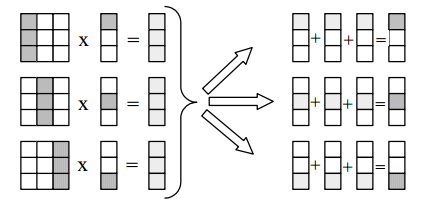
\includegraphics[width=.5\textwidth]{illustrations/matrix-vector-product/column.png}
  \caption{Computation scheme for parallel matrix-vector multiplication based on columnwise striped matrix decomposition. Note that here, we only end up with part of the (summed) $c$ vector on each process.}
  \label{fig:colwise}
\end{figure}



\subsubsection{Efficiency analysis} % (fold)
\label{ssub:efficienct_analysis}
As previously, let matrix $A$ be square, i.e. $m=n$. At the first stage of computations each processor multiplies its matrix columns by the vector $b$ elements. The obtained values are summed for each matrix row separately:
\begin{equation}
  c_s'(i) = \sum_{j=j_0}^{j_{l-1}} a_{sj}b_j, \quad 0\leq s < n
\end{equation}
where $j_0$ and $j_{l-1}$ are the initial and final column indeces of the subtasks $0\leq i <n$. As the sizes of matrix stripes and the block of the vector $b$ are equal $n/p$, the time complexity of such computations may be estimated as
\begin{equation}
  T' = \frac{n(n-1+n)}{p} \approx \frac{n^2}{p}
\end{equation}
operations. After the subtasks have exchanged the data at the second stage of computations each processor sums the obtained values up for its block of the result vector $c$. The number of the summed values for each element $c_i$ of vector $c$ conincides with the number of processors $p$. The size of result vector block is equal to $n/p$. Thus, the number of operations carried out for the second stage appears to be equal to
\begin{equation}
  T'' = \frac{n}{p} p = n
\end{equation}
Thus the total computation time is
\begin{equation}
  T_p = T' + T'' = \frac{n^2}{p} + n \approx \frac{n^2}{p}
\end{equation}
With regards to the relations obtained the speedup and the efficienct of the parallel algorithm may be expressed as follows:
\begin{equation}
  S_p = \frac{T_1}{T_p} = \frac{n^2}{n^2/p} = p, \quad E_p = \frac{T_1}{pT_p} = \frac{n^2}{p(n^2/p)} = 1
\end{equation}

Now let us consider more accurate relations for estimation of the time of parallel algorithm execution. With
regard to the above discussion the execution time of the parallel algorithm computations may be estimated by means
of the following expression:
\begin{equation}
  T_p (calc) = (\frac{n}{p}(\frac{n}{p} - 1 + \frac{n}{p}) \cdot p + \frac{n}{p} \cdot p )\tau_F
   = \left[ n (2 \frac{n}{p} -1  ) + n \right] \cdot \tau_F
\end{equation}

% subsubsection efficienct_analysis (end)



% section matrix_vector_multiplication_in_case_of_columnwise_data_decomposition (end)




% section matrix_multiplication (end)
 \clearpage


\appendix
% -*- root: ../supcom.tex -*-

\section{Exam 2013} % (fold)
\label{sec:exam_2013}
\subsection{Problem 1} % (fold)
\label{sub:problem_1}

\subsubsection{Approaches to parallelizing a program} % (fold)
\label{ssub:approaches_to_parallelizing_a_program}


\begin{question}
  \textbf{a)} We have considered two ways of parallelizing a program in the course. Outline the two different ways and explain how they relate to different hardware architectures.
\end{question}

The two primary approaches to parallelizing a program is \emph{shared memory} and \emph{distributed memory}.

\begin{description}
  \item[Shared memory:] This approach is used for systems where several processors share the same memory; i.e. all processors run in their own thread but may read from and write to the same locations in memory. The benefit of this is that the communication time between processors is eliminated. The downside is that we have to be careful when we implement the parallelization to avoid the threads overwriting eachothers buffers, causing inconsistent program output. It is also expensive if we want to use \emph{many processors}. OpenMP is a C/Fortran language extension for programming shared memory parallel machines; parallelizing programs using it is (usually) very simple.
  \item[Distributed memory:] The distributed memory approach is used for systems where each processor only has local memory access -- data stored in memory modules associated with other processes may only be accessed via explicit message passing. The most common impolementation is MPI: Message Passing Interface. This approach is more flexible than the shared memory approach, as it may also be used for processors that share memory, providing a more explicit division of memory.
\end{description}

Note that these two different implementations may be combined. E.g. for a system consisting of multiple connected nodes, where each node contains multiple processors (cores) sharing memory. MPI may then be used for communication between nodes, while OpenMP may be used to distribute the workload within each node (OpenMP may not be used across nodes).
% subsubsection approaches_to_parallelizing_a_program (end)

\subsubsection{MPI functions} % (fold)
\label{ssub:mpi_functions}


\begin{question}
  MPI is a library we have considered much in the course. It consists of more than a hundred functions. Explain how these can be grouped into four categories, and how you can use the operations from these four categories to create any communication pattern.
\end{question}

The four categores MPI functions may be grouped into are:
\begin{description}
  \item[One-to-one:] Also called point-to-point operations (send/receive). Used for communication between two specific processes.
  \item[One-to-all:] Used to distribute data from one one process to all the others, e.g. \emph{broadcast}.
  \item[All-to-one:] Used to gather data from all processes onto a root process, e.g. summing a distributed array or finding the max in it.
  \item[All-to-all:] Used to synchronize data between processes.
\end{description}
By ``all'' we mean all processes within a communicator consisting of a certain number of processes. The default is to have \emph{all} processes in the same communicator, but they may be split up.
% subsubsection mpi_functions (end)

\subsubsection{OpenMP: shared buffer} % (fold)
\label{ssub:openmp_shared_buffer}


\begin{question}
  OpenmP is another approach we have studied in the course. Consider the following piece of code
  \begin{lstlisting}
double A[5];
double b;

#pragma omp parallel for schedule(static)
for (int i=0; i<5; ++i){
  b = log(127*i/32);
  A[i] = pow(b,67);
}
  \end{lstlisting}
  Explain why the results stored in the array \texttt{A} are inconsistent between runs.
\end{question}

The results will be inconsistent because all the threads share the same memory, and therefore they all write to the same memory location when they write to the variable \texttt{b}. After one thread has written to \texttt{b}, and before it has written to \texttt{A[i]}, some other thread may have written its own (different) value to the memory location, thus changing the ``intended'' content of \texttt{A[i]}. The threads are run in no particular order, so the content of \texttt{A}  will vary from run to run.
% subsubsection openmp_shared_buffer (end)

\subsubsection{MPI-I/O} % (fold)
\label{ssub:mpi_i_o}


\begin{question}
  Explain how you can use MPI-I/O to store a multi-dimensional, parallel array to disk in a single operation.
\end{question}

To store a multi-dimensional, parallel array to disk in a single operation using MPI-I/O, we first need to define a communicator with an attached topology (e.g. cartesian), and map the processes onto it. We then create a custom datatype describing the data pattern on secondary storage, a file view with this attached. We can then use this file view when we call the write function on each process.

Because the system knows the data access patterns on each process up front, it can optimize how storing the data to disk is performed.
% subsubsection mpi_i_o (end)
% subsection problem_1 (end)




\clearpage
\subsection{Problem 2} % (fold)
\label{sub:problem_2}


\begin{question}
  We here consider the solution of a 2D Helmholtz problem with homogenous Dirichlet boundary conditions on the unit square;

  \begin{equation}
    - \nabla^2 u + \mu u = f \; \text{in} \; \Omega = (0,1) \times (0,1), \; u\vert_{\partial \Omega}
  \end{equation}

  The problem is discretized using finite difference methods, with the five point formula for the second derivatives on a structured mesh with spacing $h=1/n$ in both spatial directions. This results in the linear system of equations

  \begin{equation}
    \mathbf{A}u=f
  \end{equation}
\end{question}

\subsubsection{Gauss-Jacobi using functions} % (fold)
\label{ssub:gauss_jacobi_using_functions}


\begin{question}
  Explain why and how you can avoid forming the matrix if you employ Gauss-Jacobi iterations to solve this problem.
\end{question}

\begin{equation}
  x_i^{k+1} = \frac{1}{a_{ii}} \left( b_i - \sum_{j=1, j\neq i}^N a_{ij} x_j^k \right) \label{eq:gauss_seidel}
\end{equation}

As we se from the formula used for Gauss-Jacobi iterations over, the method does no require changing the matrix $\mathbb{A}$; only the values in the vector $u$ are updated. This, combined with the fact that the five-point stencil will give us a fairly simple banded matrix $\mathbf{A}$ with five diagonals and all known values, implies that we can easily get the values for each required pair of $i,j$ in $A_{ij}$ using a simple function.
% subsubsection gauss_jacobi_using_functions (end)

\subsubsection{Hybrid MPI/OpenMP solver for the Gauss-Jacobi scheme} % (fold)
\label{ssub:hybrid_mpi_openmp_solver_for_the_gauss_jacobi_scheme}
We can use domain decomposition to divide the problem across multiple processes. I.e. each process computes a specific set of rows. In each process we can then use OpenMP to further divide the row computations across threads. We will still need some computed $u$ values from the other processes; these are exchanged using MPI\_Shift and MPI\_Sendrecv.

Finally we can simply gather the computed $u$ vector on the root process.
% subsubsection hybrid_mpi_openmp_solver_for_the_gauss_jacobi_scheme (end)

\subsubsection{Speedup and efficiency} % (fold)
\label{ssub:speedup_and_efficiency}


\begin{question}
  Give parallel speedup and efficiency estimates. You can assume a simple linear network model:
  \begin{equation}
    \nonumber
    \tau = \tau_s + m\tau_c
  \end{equation}
  where $\tau$ is the total time; $\tau_s$ is the latency; $\tau_c$ is the inverse bandwidth of the network (i.e. time pr. byte); and $m$ is the number of bytes sent. We have to perform $M$ iterations to reduce the residual sufficiently. You can ignore the use of threads in this calculation, and you can assume that $n \gg 1$ .
\end{question}

From \eqref{eq:gauss_seidel} we see that each iteration for our system looks (with the five-point stencil) that we will get
\begin{itemize}
  \item 1 division: $\frac{1}{a_ii}\times(\dots)$.
  \item 1 subtraction: $b_i - \sum[\dots]$.
  \item 4 multiplications: $a_{ij}x_j^k$ is performed for the four non-zero off-diagonal elements pr. row; not for the element on the diagonal because of the $j\neq i$.
  \item 3 additions: four $a_{ij}x_j^k$ elements are summed.
\end{itemize}
in total 9 operations. The time required to do each operation, i.e. one flop, is $\tau_f$. These 9 operations are performed $n^2$ times (we're operating in 2D, so we have $n^2$ equations). And so the total time required to do one sweep is
\begin{equation}
  T_1^s = 9n^2\tau_f
\end{equation}
We then need to compute the resudial $r$ to check the convergence criterium. This is computed as
\begin{equation}
  r = b - \mathbf{A}x^k
\end{equation}
which requires the following operations:
\begin{itemize}
  \item For $\mathbf{A}x^k$ we need $n^2$ multiplications and $n(n-1)$ addtions. $n^2+n(n-1)\asymp 2n^2$.
  \item For $b - \mathbf{A}x^k$ we need $n$ subtractions.
\end{itemize}
Asymptotically we need $2n^2 + n \asymp 2n^2$ operations to perform the convergence criterium check. Therefore the total time required pr. iteration is
\begin{equation}
  T_1 = T_1^s + 2n^2 \tau_f = 11n^2 \tau_f
\end{equation}

% TODO: Gjør ferdig dette

% subsubsection speedup_and_efficiency (end)

% subsection problem_2 (end)



\clearpage
\subsection{Problem 3} % (fold)
\label{sub:problem_3}

\subsubsection{Applicability of the FST Poisson solver} % (fold)
\label{ssub:applicability_of_fst}


\begin{question}
  The fast sine transform based Poisson solver considered in the course is aplicable to any elliptic equation. \textbf{True/False}.
\end{question}

\textbf{False}. The \emph{diagonalization} method; to use \emph{FST} we depend on the particular eigenspace of the Poisson matrix -- it needs to be periodic with period $2\pi$ and \emph{odd}.
% subsubsection applicability_of_fst (end)

\subsubsection{MPI vs. OpenMP} % (fold)
\label{ssub:mpi_vs_openmp}


\begin{question}
  Eventually, OpenMP will replace MPI as the preferred standard for parallel computing. \textbf{True/False}.
\end{question}

\textbf{False}. OpenMP and MPI supplement eachother, they do not replace eachother. Both the distributed and shared memory models will be around in the forseeable future.
% subsubsection mpi_vs_openmp (end)

\subsubsection{Smallest number: \texttt{float} vs \texttt{double}} % (fold)
\label{ssub:smallest_number_tt}

\begin{question}
  You can represent smaller numbers using double precision than single precision. \textbf{True/False}.
\end{question}

\textbf{True}. Each floating point has a binary representation with three fields: $S$, denoting the sign; $E$ is the exponent; and $F$ is the fraction part of the mantissa:

\vspace{1em}

\begin{center}
  \begin{tabular}{|c|c|c|}
    \hline
    S & \hspace{4em} E \hspace{4em} & \hspace{8em} F \hspace{8em} \\
    \hline
  \end{tabular}
\end{center}

The actual value of the floating point is
\begin{equation}
  V = (-1)^S \cdot 2^{E-B} \cdot M \label{eq:float_value}
\end{equation}
where $M$ is the mantissa, and $B$ is called the \emph{bias}. The exponent $E$ is always adjusted such that the mantissa can be expressed as
\begin{equation}
  M = \underset{\times 2^0}{\underbrace{1}} \, . \,
                                              \overset{F}{
                                                \overbrace{
                                                  \underset{\times 2^{-1}}{\underbrace{b_1}} \;
                                                  \underset{\times 2^{-2}}{\underbrace{b_2}} \;
                                                  \underset{\times 2^{-3}}{\underbrace{b_3}} \;
                                                  \dots
                                                }
                                              }
\end{equation}
where $F$ denotes the fraction of the mantissa in binary representation. (i.e.) the binary digits $b_1b_1\dots$. Since this representation is always assumed, the binary number 1 in the front is not explicitly represented. Note that, in decimal representation,
\begin{equation}
  1 \leq M < 2
\end{equation}
since the fraction $F$ in decimal representation is always less than 1.

The number of bytes used for each part for single- and double precision floats are shown in the table below.

\vspace*{1em}
\begin{center}
    \begin{tabular}{lllll|l}
      \toprule
      \textsc{Precision} & $S$ & $E$ & $F$ & \textsc{Total} & \textsc{Bias} \\
      \midrule
      Single & 1 & 8  & 23 & 32 & 127 \\
      Double & 1 & 11 & 52 & 64 & 1023 \\
      \bottomrule
  \end{tabular}
\end{center}

In single precision, $E$ is represented using 8 bits, giving $2^8 = 256$ possibilities (including 0) where the values $E=0$ and $E=255$ are used to represent zero and infinity, respectively. Which means that the smallest and largest $E$'s used for representing other numbers are $E_{min,s}=1$ and $E_{max,s}=254$.

For double precision, $E$ is represented using 11 bits, giving $2^{11}=2048$ possibilities. Again, $E=0$ is reserved for zero and $E=2048$ is reserved for infinity. Which means that the largest avalable exponent is $E_{max,d}=2046$.

For both double and single precision, the largest possible mantissa is $M=1.999\dots \approx 2$. Combining these maximum values for $M$ and $E$ with $S=1$ and the bias $B$ in equation \eqref{eq:float_value} gives us the largest negative numbers for single and double precision numbers:
\begin{align}
    V_{min_1, s} &= (-1)^1 \cdot 2^{254-127} \cdot 2 = -3.40\dots\times 10^{38} \\
    V_{min_1, d} &= (-1)^1 \cdot 2^{2046-1023} \cdot 2 = 1.7\dots \times 10^{308}
\end{align}

If we interpret ``smallest'' value as the number with the smallest absolute value (or the smallest fraction), then we need the smallest value for the mantissa and the largest negative value for the exponent. These are, respectively, $M_{min} = 1, E_{min} = 1$. So the smallest numbers for double and single precision are
\begin{align}
    V_{min_2, s} &= 1 \cdot 2^{1-127} \cdot 1 = 1.17\dots \times 10^{-38}
    V_{min_2, d} &= 1 \cdot 2^{1-1023} \cdot 1 = 2.22\dots \times 10^{-308}
\end{align}

So we see that, whichever way we enterpret ``smallest number'', double precision will give us a smaller number.

\vspace*{1em}\noindent \textbf{\emph{Note on accuracy}}: By accuracy we mean the smalles fraction that can be represented by the mantissa. This is given by the number of bytes that are used by the format to store the matissa $F$. For single precision, this is 23; so the smallest fraction we can represent is $2^{-23} = 1.19\dots \times 10^{-7}$. This implies that we have about 7 digits of accuracy. For double precision numbers we use 52 bits to store the mantissa, so the smallest fraction we can represent is $2^{-52}=2.22\dots \times 10^{-16}$. This implies that doubles have about 16 digits of accuracy.
% subsubsection smallest_number_tt (end)

\subsubsection{Cancellation} % (fold)
\label{ssub:cancellation}


\begin{question}
  Cancellation is a concern when adding floating point numbers. \textbf{True/False}.
\end{question}

\textbf{False}. Cancellation happens when you \emph{subtract} numbers that are very close.
% subsubsection cancellation (end)

\subsubsection{N-way cache} % (fold)
\label{ssub:n_way_cache}


\begin{question}
  Processors with N-way cache cannot be superscalar.
\end{question}
\textbf{False}. A processor can be superscalar no matter the cache layout. N-way cache mapping is illustrated in Figure~\ref{fig:nway}. When we use $n$-way cahce mapping, there are $n$ ways to map a memory address to a cache address, i.e. a particular memory location can potentially end up in one of $n$ cache lines (Figure~\ref{fig:nway}). This means fewer cache misses (compared to direct mapping), thus increasing the possibility of keeping the pipe filled, which increases the superscalar performace.

\begin{figure}[htbp]
  \centering
  \includegraphics[]{illustrations/cache/n-way.pdf}
  \caption{$n$-way set-associative cache.}
  \label{fig:nway}
\end{figure}
% subsubsection n_way_cache (end)

\subsubsection{OpenMP scheduling} % (fold)
\label{ssub:openmp_scheduling}


\begin{question}
  A code consists of a \texttt{for}-loop with a big difference in cost between each iteration. If we are to do this loop in parallel using OpenMP, a ``guided'' scheduling mode is a good choice. \textbf{True/False.}
\end{question}

\emph{True}. A guided mode will likely give the best balance, given that there is no bias (that the cost does not depend on iteration). If there is a bias, guided will give the heaviest calculations to the first threads, which means that the later threads may finish before them. In that case, dynamic will be better.
% subsubsection openmp_scheduling (end)

\subsubsection{Parallel performance vs. code optimization} % (fold)
\label{ssub:parallel_performance_vs_code_optimization}


\begin{question}
  It is easier to get good parallel efficiency on a well-optimized code. \textbf{True/False}.
\end{question}

\textbf{False}. Typically you get a better efficiency on less optimized code since the balance between communication and computation has shifted (communication is more relevant). Optimizing for communication is often easier to do on code that has not already been optimized for computation.
% subsubsection parallel_performance_vs_code_optimization (end)

\subsubsection{Generality of domain decomposition} % (fold)
\label{ssub:generality_of_domain_decomposition}


\begin{question}
  When solving a linear system of equations, domain decomposition methods are preferred in parallel due to the generality. \textbf{True/False}.
\end{question}

\textbf{False}. They are prefered due to their ability to reduce network traffic. A method based on matrix distribution would be more general.

% subsubsection generality_of_domain_decomposition (end)


% subsection problem_3 (end)

% section exam_2013 (end)
 \clearpage
% -*- root: ../supcom.tex -*-

\section{Exam 2012} % (fold)
\label{sec:exam_2012}

\subsection{Problem 1} % (fold)
\label{sub:problem_1}


\begin{question}
  Consider the solution of the linear system of equations
  \begin{equation}
    \mathbf{Ax} = \mathbf{b} \label{eq:3dpoissonmat}
  \end{equation}
  where $\mathbf{A}$ is a $(n-1)^3 \times (n-1)^3$ matrix and $\mathbf{b}$ is a vector of length $(n-1)^3$. Here $\mathbf{A}$ originates from the discretization of a $3D$ Poisson problem with homogenous Dirichet boundary conditions, using a centered difference approach on a grid with $n+1$ grid points in each direction; see Figure~\ref{fig:3d-stencil}. The unknowns are numbered in a natural order running fastest along the $x$ direction. For implicity we also introduce number of degrees of freedom in each spatial direction;
  \begin{equation}
    m = n-1 \label{eq:3dpoisson_degrees_of_freedom}
  \end{equation}
  The resulting matrix will have a bandwidth
  \begin{equation}
    b = m^2 \label{eq:3dpoisson_bandwidth}
  \end{equation}

  \begin{figure}[H]
    \centering
    \includegraphics[scale=0.5]{illustrations/stencils/3d-center.pdf}
    \caption{The stencil used to form \eqref{eq:3dpoissonmat}.}
    \label{fig:3d-stencil}
  \end{figure}
\end{question}


\subsubsection{Memory requirement: LU-decomposition} % (fold)
\label{ssub:memory_requirement_lu_decomposition}


\begin{question}
  Let $n=30$. Assuming we use dense matrices and full LU-decomposition, what is the approximate memory requirement? All numbers are stored in double precision.
\end{question}
We need to store 3 full matrices, $\mathbf{A}$, $\mathbf{L}$ and $\mathbf{U}$, the \emph{load vector} $\mathbf{b}$, as well as solution vector $\mathbf{x}$. All the three full matrices are of size
\[
  M_A = M_L = M_U = (n-3)^3\times (n-1)^3 = m^3\times m^3 = m^6
\]
while the vectors are of size
\[
  M_b = M_x = (n-1)^3 = m^3
\]
so the total memory requirement (given that all numbers are doubles) is
\begin{equation}
  M_{tot} = \left( 3m^6 + 2m^3 \right) \times 8 \approx 14 \mathrm{GB}
\end{equation}
% subsubsection memory_requirement_lu_decomposition (end)


\subsubsection{Memory requirement: Banded Cholesky} % (fold)
\label{ssub:memory_requirement_banded_cholesky}


\begin{question}
  If we instead use a banded Cholesky approach, what is the expected memory usage?
\end{question}
% subsubsection memory_requirement_banded_cholesky (end)


\subsubsection{FLOP per iteration} % (fold)
\label{ssub:flop_per_iteration}


\begin{question}
  Give an estimate of the required number of FLOP (per iteration) if we employ a preconditioned conjugate gradient method. You can assume that we use a solver package that gives us access to a very efficient, diagonal preconditioner, which requires 1 flop/unknown. You can ignore any boundary effects.
\end{question}
% subsubsection flop_per_iteration (end)


\subsubsection{Parallel computation time} % (fold)
\label{ssub:parallel_computation_time}

\begin{question}
  The machine we have access to to solve \eqref{eq:3dpoissonmat} has a slow network on \emph{only allows for a pure distributed memory model}. You can assume a simple network model where the time to send $k$ bytes over the network, $\tau_c(k)$ can be estimated as
  \begin{equation}
    \tau_c(k) = \tau_s + \gamma \cdot k
  \end{equation}
  where $\tau_s$ is a startup time and $\gamma$ is the inverse bandwidth.
  \[
    \tau_s = 10^{-4}\mathrm{s} \; \gamma = 10^{-7}\mathrm{s/byte}
  \]

  We also assume a very simple model for the computation times, and assume that we get 50\% of the full superscalar behaviour of the processors, which runs at 2.4GHz.

  The time restriction is \emph{10 seconds}, and we can use \emph{64 processors}. The algorithm in use is the preconditioned conjugate gradient (CG) method mentioned earlier, in combination with domain decomposition.

  Using the diagonal preconditioner, we need 10 iterations to reach an acceptable tolerance. You can still ignore any boundary effects.

  What is the largest problem size we can run?
\end{question}

% subsubsection parallel_computation_time (end)

% subsection problem_1 (end)

\clearpage
\subsection{Problem 2} % (fold)
\label{sub:problem_2}


\begin{question}
  Assume that you are given $\mathbf{L}$, which is some general, full matrix (no sparsity can be expected) of dimension $N\times N$. We are then asked to perform the matrix-vector product
  \begin{equation}
    \mathbf{u} = \mathbf{Lx}
  \end{equation}
  for some (given) vector x.
\end{question}

\subsubsection{Partitioning} % (fold)
\label{ssub:partitioning}


\begin{question}
  Outline the different ways we can partition the matrix in a distributed memory setting.
\end{question}

\noindent There are two basic approaces: either strips (rows or columns) or blocks.

\begin{center}
  \includegraphics[width=\textwidth]{illustrations/io/splitting.pdf}
\end{center}
% subsubsection partitioning (end)


\subsubsection{Parallel computation of matrix-vector product} % (fold)
\label{ssub:parallel_computation_of_matrix_vector_product}


\begin{question}
  Outline how you would perform the matrix-matrix product for the different partitioning approaches. Which of these methods do you think is the most efficient? Consider both the number of FLOP required and the communication time (you can use the network model from task 1). Is any of the partitioning approaches peferable with a hybrid model?

  \noindent Communication model:
  \begin{itemize} \itemsep=0em
    \item Time to send $k$ bytes: $\tau_c(k) = \tau_s + \gamma \cdot k$
    \item Startup time: $\tau_s = 10^{-4}$s
    \item Inverse bandwidth: $\gamma = 10^{-7}$s/byte
  \end{itemize}

\end{question}

\noindent \textbf{Generally:} Assuming that

\noindent\textbf{Row-based strip partitioning:}

\begin{itemize}
  \item $\mathbf{A}$ is distributed across the processes.
  \item The entire vector $\mathbf{x}$ needs to be collected on every process $P_i$.
  \item $\mathbf{Ax}$ is performed locally on each process $P_i$ to form part $u_i$ of the solution vector $\mathbf{u}$.
  \item Finally the solution vector $\mathbf{u}$ must be collected.
\end{itemize}

\begin{center}
  \includegraphics[]{illustrations/partitioning/strip-row.pdf}
\end{center}

\noindent \emph{FLOPs required:} Each of the $N$ rows requires $N$ multiplications and $N-1$ additions.
\[
  FLOP_{row} = N ( N + (N-1) ) = 2N^2 - N
\]

\noindent \emph{Communication time:} In the startup phase we need to distribute the $N\times N$ elements in $\mathbf{A}$ to $P$ different processors:
\[
  \tau_{start} = P\tau_c(N^2/P) = P \left( \tau_s + \frac{N^2}{P} \gamma \right) = P\tau_s + N^2 \gamma
\]
At the end we need to gather the $N$ elements in the solution vector $\mathbf{u}$ to one process:
\[
  \tau_{end} = P\tau_c(N/P) = P \left( \tau_s + \frac{N}{P} \gamma \right) = P\tau_s + N\gamma
\]
So in total we have
\[
  \tau_{total,row} = 2P\tau_s + \gamma(N+N^2)
\]



\noindent\textbf{Column-based strip partitioning:}

\begin{itemize}
  \item $\mathbf{A}$ and $\mathbf{x}$ is divided across the processes. I.e. each process gets $N/P$ columns from $\mathbf{A}$ and $N/P$ rows from $\mathbf{x}$.
  \item $\mathbf{Ax}$ is performed locally on each process to form part of the product.
  \item Sum the computed parts from each process to get the final result (N/P summations).
\end{itemize}

\begin{center}
  \includegraphics[]{illustrations/partitioning/strip-col.pdf}
\end{center}

\noindent \emph{FLOPs required:} Each of $N$ rows require $N$ multiplications and $N-1$ additions. Additionally, we need to perform ($P-1$) additions per row.
\[
  FLOP_{col} =  N ( N + (N-1) ) + N( P-1 ) = 2N^2  - 2N + NP
\]

\noindent \emph{Communication time:} In the startup phase we need to distribute the $N\times N$ elements in $\mathbf{A}$ to $P$ different processors. We also need to divide the $N$ elements in the vector $\mathbf{x}$ across them.
\[
  \tau_{start} = P\tau_c((N^2+N)/P) = P \left( \tau_s + \frac{N^2+N}{P} \gamma \right) = 2P\tau_s + \gamma(N+N^2)
\]
At the end we need to sum the partly computed product from each of the $P$ processes:
\[
  \tau_{end} = (P-1)\tau_c(N/P) = (P-1) \left( \tau_s + \frac{N}{P} \gamma \right) = (P-1)\tau_s + N\gamma
\]
So in total we have
\[
  \tau_{total,col} = 3P\tau_s + \gamma(2N+N^2)
\]


\noindent\textbf{Block-based partitioning:}

\begin{itemize}
  \item Combination of the two approaches above.
  \item The matrix $\mathbf{A}$ is divided across the processes. Each process also gets part of the vector $\mathbf{x}$: processes $P_0, P_3, P_6$ gets part $x_0$, processes $P_1, P_4, P_7$ gets part $x_1$, etc.
  \item $\mathbf{Ax}$ is performed locally on each process.
  \item The rows from $P_0, P_1, P_2$ are summed to form solution part $u_0$, rows from $P_3, P_4, P_5$ are summed to form solution part $u_1$, etc.
  \item Finally the solution vector $\mathbf{u}$ must be collected.
\end{itemize}

\begin{center}
  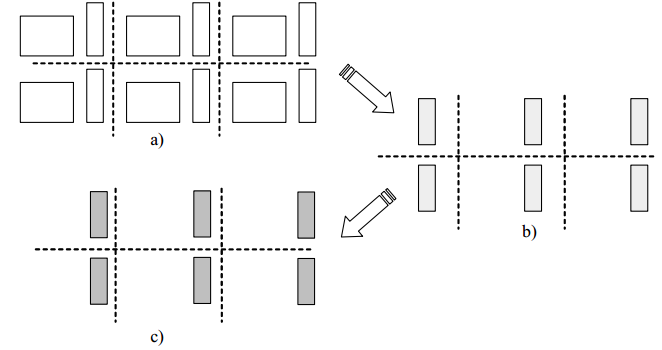
\includegraphics[]{illustrations/partitioning/block.pdf}
\end{center}

\noindent \emph{FLOPs required:} Each of $N$ rows require $N$ multiplications and $N-1$ additions. Additionally, we need to perform one ($\sqrt{P}-1$) additions per row.
\[
  FLOP_{block} =  N ( N + (N-1) ) + N( \sqrt{P}-1 ) = 2N^2  - 2N + N \sqrt{P}
\]

\noindent \emph{Communication time:} In the startup phase we need to distribute the $N\times N$ elements in $\mathbf{A}$ to $P$ different processors. We also need to divide the $N$ elements in the vector $\mathbf{x}$ across them.
\[
  \tau_{start} = P\tau_c((N^2+N)/P) = P \left( \tau_s + \frac{N^2+N}{P} \gamma \right) = 2P\tau_s + \gamma(N+N^2)
\]
At the end we need to sum the partly computed product from each row of blocks:
\[
  \tau_{end} = (\sqrt{P}-1) \tau_c(N/(\sqrt{P}-1)) = (\sqrt{P}-1) \left( \tau_s + \frac{N}{\sqrt{P}-1} \gamma \right) = (\sqrt{P}-1)\tau_s + (\sqrt{P}-1)N\gamma
\]
So in total we have
\[
  \tau_{total,block} = (2P+\sqrt{P}-1)\tau_s + \gamma(N+N^2+(\sqrt{P}-1)N)
\]

\noindent \textbf{Comparison:} Using the numers from the previous problem: $P=64$, $f=2.4$ GHz, $m=30,100,1000,1500$. The equation for computation time is
\[
  \tau_{comp} = \frac{FLOP}{f}
\]

\begin{center}
  \begin{tabular}{ll|lll}
    \toprule
    \textsc{Approach} & $N$ & \textsc{Comm}& \textsc{Comp}  & \textsc{Tot} \\
    \midrule
    Row    & 30    & 0.012893 & 7.3750e-07 & 0.012894 \\
           & 100   & 0.013810 & 8.2917e-06 & 0.013818 \\
           & 1000  & 0.112900 & 8.3292e-04 & 0.113733 \\
           & 1500  & 0.237950 & 1.8744e-03 & 0.239824 \\
           & 20000 & 40.01480 & 0.33332    & 40.34812 \\
    \midrule
    Column & 30    & 0.019296 & 1.5250e-06 & 0.019298 \\
           & 100   & 0.020220 & 1.0917e-05 & 0.020231 \\
           & 1000  & 0.119400 & 8.5917e-04 & 0.120259 \\
           & 1500  & 0.244500 & 1.9138e-03 & 0.246414 \\
           & 20000 & 40.02320 & 0.33385   & 40.35705 \\
    \midrule
    Block  & 30    & 0.013614 & 8.2500e-07 & 0.013615 \\
           & 100   & 0.014580 & 8.5833e-06 & 0.014589 \\
           & 1000  & 0.114300 & 8.3583e-04 & 0.115136 \\
           & 1500  & 0.239700 & 1.8787e-03 & 0.241579 \\
           & 20000 & 40.02950 & 0.33338    & 40.36288 \\
    \bottomrule
  \end{tabular}
\end{center}

With numbers inserted, we can see that there is almost no difference in computation time. The communication time becomes extremely dominant for all cases, implying that the use of shared memory parallelization using OpenMP in combination with MPI would be a large improvement.

Depending on the number of cores used for shared memory computation, row based would be best for few cores, while column or block-based would be better for many.
% subsubsection parallel_computation_of_matrix_vector_product (end)
% subsection problem_2 (end)



\clearpage
\subsection{Problem 3: True/False} % (fold)
\label{sub:problem_3}

\begin{question}
  An $n$-way associative cache is much more prone to cache trashing.
\end{question}
\textbf{False.} It is much less prone to cache trashing because all memory locations can be mapped to $n$ different cache lines.

\vskip2em
\begin{question}
  Dense $LU$ factorization is useless for large systems due to the low FLOPS.
\end{question}
\textbf{False.} It gives close to optimal FLOPS. It is unusable for larger systems due to the amount of operations required, not the speed they are performed at.

\vskip2em
\begin{question}
  If your program is compute bound, a shared memory implementation can be faster than a distributed memory implementation.
\end{question}
\textbf{True.} If memory is not an issue a shared memory implementation will be faster, because a distributed memory implementation would incur communication time. It will also benefit from better cache usage.


\vskip2em
\begin{question}
  The conjugate gradient method is a direct solution method.
\end{question}
\textbf{False.} In general it is considered to be an iterative method. Although it may be considered direct if only exact arithmetics are involved, as it will then only require $n$ iterations.

\vskip2em
\begin{question}
  The BLAS and LAPACK libraries generally work with row-major matrix formats.
\end{question}
\textbf{False.} They are implemented in -- and originally designed for -- FORTRAN, which is column-major.

\vskip2em
\begin{question}
  CMake is used to build a program.
\end{question}
\textbf{False.} CMake are used to generate a build system (e.g. makefiles), which are in turn used to build a program.

\vskip2em
\begin{question}
  If we do parallel Monte-Carlo simulations, it is imperative to know the period of the PRNG (Pseudo Random Number Generator) to avoid doing the same simulations several times within a single process.
\end{question}
\textbf{True.} The period tells us how many simulations we can do on a single process before the sequence repeats. The seed is what ensures different simulations are done on the different processes.

\vskip2em
\begin{question}
  The fast diagonalization method considered in the course is optimal in sense of the number of FLOP required. Hint: optimal has a particular meaning in the context!
\end{question}
\textbf{False.} The method is $O(N^2 \log_2 N)$, i.e. we use $\log_2 N$ operations per degree of freedom; $N$ would be optimal.

% subsection problem_3 (end)

% section exam_2012 (end)
 \clearpage
% -*- root: ../supcom.tex -*-

\section{Exam 2011} % (fold)
\label{sec:exam_2011}

\subsection{Problem 1: Matrix-matrix multiplication and BLAS} % (fold)
\label{sub:problem_1}

\begin{question}
  Let $\mathbf{a}$ and $\mathbf{b}$ be real vectors of length $n$, and $\mathbf{A}$, $\mathbf{B}$ and $\mathbf{C}$ be real $n\times n$ matrices. Consider the innerproduct (or dot product)
  \begin{equation}
    \sigma = \mathbf{a}^T \mathbf{b} = \mathbf{a} \cdot \mathbf{b}
  \end{equation}

  and the matrix-matrix multiplication
  \begin{equation}
    \mathbf{C} = \mathbf{AB}
  \end{equation}

  We recall that each matrix element $c_{ij}$ of $\mathbf{C}$ can be expressed as the innerproduct between the $i$-th row of $\mathbf{A}$ and the $j$-th column of $\mathbf{B}$, i.e. one innerproduct per matrix element.
\end{question}

\subsubsection{Matrix-matrix multiplication computation time, using BLAS Level 1} % (fold)
\label{ssub:matrix_matrix_multiplication_computation_time}

\begin{question}
  First, we implement the matrix-matrix multiplication on a single processor using a fast implementation fo the innerproduct operation (e.g. using Level 1 BLAS). Timing of the matrix-matrix product with $n=1000$ yields an average time per innerproduct equal to $1.0\times 10^{-5}$ seconds. What is the time to perform the matrix-matrix product for this implementation? What is the corresponding performance in terms of the number of FLOPS?
\end{question}

The matrix-matrix operation consists of $n\times n$ inner products, each taking $10^{-5}$ seconds to perform. So the time to perform all the inner products is
\begin{equation}
  T_{m\times m} = n^2 10^{-5} = 10 s
\end{equation}

Each inner product requires $n-1$ additions and $n$ multiplications, and we need to do $n^2$ inner products. To the total number of operations required are
\begin{equation}
  N_{m\times m} = n^2((n-1)+n) \approx 2n^3 = 2 \times 10^9
\end{equation}
so the number of FLOPS is
\begin{equation}
  FLOPS_{m\times m} = \frac{N_{m\times m}}{T_{m\times m}} = 200\times 10^6 = 200 \mathrm{Mflops}
\end{equation}

% subsubsection matrix_matrix_multiplication_computation_time (end)


\subsubsection{Matrix-matrix multiplication computation time, using BLAS Level 3} % (fold)
\label{ssub:matrix_matrix_multiplication_computation_time_using_blas_level_3}

\begin{question}
  Next, we implement the matrix-matrix product using Level 3 BLAS. The performance is measured to be 6 Gflops for $n=1000$. What is the time to perform the matrix-matrix multiplication for this implementation? Does this seem reasonable compared to the result in the previous implementation?
\end{question}

We still need to perform $2n^3$ operations. We can perform $6\times 10^9$ operations per second. The time to perform the operations is
\begin{equation}
  \frac{2n^3}{6\times 10^9} = \frac{1}{3} s
\end{equation}

The results seem reasonable: Level 3 BLAS operations exploit the computational resources much better than level 1 because of better data reuse. This means that we can use the cache more, and reduces the memory traffic significantly compared to level 1 operations.

We typically get fairly close to maximum theoretical performance using Level 3 BLAS.

% subsubsection matrix_matrix_multiplication_computation_time_using_blas_level_2 (end)

% subsection problem_1 (end)



\subsection{Problem 2: The Poisson problem -- Conjugate gradient method and grid partitioning} % (fold)
\label{sub:problem_2}

\begin{question}
  We would like to solve the Poisson problem on the unit square $\Omega = (0,1) \times (0,1)$ with boundary conditions $u=0$ specified alon the boundary $\partial \Omega$. We discretize the problem using finite difference techniques; the Laplace operator is approximated using the standard 5-point stencil. The grid spacing in each spatial direction is $h=1/n$, where $n\gg 1$.

  The Conjugate gradient method is used to solve the system of algebraic equations. The implementation is done in double precision. In the multi-processor case, the original grid is decomposed into $P$ approximately equal subgrids, each of size $m\times m$, i.e. $m^2 \approx n^2/P$ (i.e. we slice the grid both in $x$- and $y$-direction). We assign one subgrid to each processor.

  In the following, you can assume that the time it takes to send a message of $k$ bytes over the network can be expressed as
  \begin{equation}
    \tau_C(k) = \tau_S + \gamma k
  \end{equation}
  where $\tau_S$ is the startup time and $\gamma$ is the inverse bandwidth.
\end{question}

\subsection{Communication cost per conjugate gradient iteration} % (fold)
\label{sub:communication_cost_per_conjugate_gradient_iteration}

\begin{question}
  Give an expression for the communication cost per conjugate gradient iteration.
\end{question}

The algorithm for the conjugate gradient method is as follows:

\begin{algorithm}[H]
  \SetKwInput{KwSet}{Set}
  \KwSet{$\mathbf{u}^0=\mathbf{0}, \mathbf{r}^0=\mathbf{f}$}
  \For{$m=1,2,...$}{
    $\beta_{m}=\frac{\left(\mathbf{r}^{m-1}\right)^{T}\mathbf{r}^{m-1}}{\left(\mathbf{r}^{m-2}\right)^{T}\boldsymbol{r}^{m-2}}\qquad\qquad(\beta_{1}\equiv0)$ \;
    $\boldsymbol{p}^{m}=\boldsymbol{r}^{m-1}+\beta_{m}\boldsymbol{p}^{m-1}\qquad(\boldsymbol{p}^{1}\equiv\boldsymbol{r}^{0})$ \;
    $\alpha_{m}=\frac{\left(\boldsymbol{r}^{m-1}\right)^{T}\boldsymbol{r}^{m-1}}{\left(\boldsymbol{p}^{m}\right)^{T}\boldsymbol{A}\boldsymbol{p}^{m}}$ \;
    $\boldsymbol{u}^{m}=\boldsymbol{u}^{m-1}+\alpha_{m}\boldsymbol{p}^{m}$ \;
    $\boldsymbol{r}^{m}=\boldsymbol{r}^{m-1}-\alpha_{m}\boldsymbol{A}\boldsymbol{p}^{m}$ \;
  }
  \caption{The conjugate gradient method.}
\end{algorithm}

% subsection communication_cost_per_conjugate_gradient_iteration (end)

% subsection problem_2 (end)

% section exam_2011 (end)
 \clearpage
% -*- root: ../supcom.tex -*-

\section{Exam 2006} % (fold)
\label{sec:exam_2006}

\subsection{Problem 1: Inner product} % (fold)
\label{sub:problem_1_inner_product}

\begin{question}
  Let $x$ and $y$ be two vectors of length $n$. Consider the following operations (innerproducts):

  \begin{align}
    \sigma_1 &= x^T x = \sum_{i=1}^n x_i \cdot x_i \label{eq:2006_1_1} \\
    \sigma_2 &= x^T y = \sum_{i=1}^n x_i \cdot y_i \label{eq:2006_1_2}
  \end{align}
  Both operations are to be computed numerically in double precision on $P$ processors. Note that operation \eqref{eq:2006_1_1} is the same as operation \eqref{eq:2006_1_2} when $x=y$.

  Assume in the following that each processor is a MIPS processor of the same type as on gridur. The clock frequency is 500 MHz and at the most a single floating point can be transferred to or from the memory per clock cycle. Assume further that we use a distributed memory multiprocessor machine with the following network characteristics: the time it takes to send a message with $k$ bytes, $\tau_C(k)$ can be approximated as
  \begin{equation}
    \tau_C(k) = \tau_S + \gamma k
  \end{equation}
  Here, $\tau_S$ is a fixed startup time and $\gamma$ is the inverse bandwidth.
\end{question}

\subsubsection{Expected maximum performance} % (fold)
\label{ssub:expected_maximum_performance}

\begin{question}
  We consider first the single processor case $P=1$. What is the expeced maximum performance of operation \eqref{eq:2006_1_1} and operation \eqref{eq:2006_1_2}? How great is this performance compared to the maximum theoretical performance for this type of processor?
\end{question}

Pipelining and chaining allows the processor to, after some startup time, perform \emph{two} FLOPs (multiply-add) per clock cycle, meaning that the maximum theoretical performance of the processor is $2\times 500 Mflops=1 Gflops$.

For the inner product operation \eqref{eq:2006_1_2}, the performance is memory bound. While we accumulate the constributions in the variable $\sigma$, this variable can be stored in the register. In order to update $\sigma$ with the next $x_i \cdot y_i$ contribution, we need to get the two new components from memory; this will take two clock cycles. During these two clock cycles we can, using pipelining and chaining, perform the multiply-add for the previous two loaded elements. Thus we are able to perform two FLOPs per two clock cycles, or 50\% of the maximum theoretical performance. This performance can be (approximately) seen for problems where the vectors $x$ and $y$ are fully available in the L1 cache.

For the innerproduct operation \eqref{eq:2006_1_1} only a single memory reference is needed for each $\sigma$ contribution $x_i\cdot x_i$; we can get this in one clock cycle. During this clock cycle we can perform the multiply-add operation (two flops) for the previous element retrieved from memory. This performance corresponds to the maximum theoretical performance, 1 Gflops. This performance can be (approximately) seen for problems where the vectors $x$ and $y$ are fully available in the L1 cache.

% subsubsection expected_maximum_performance (end)

\subsubsection{Expected multiprocessor performance} % (fold)
\label{ssub:expected_multiprocessor_performance}

\begin{question}
  We now consider the multiprocessor case ($P>1$). Assume that the vectors $x$ and $y$ are aleady distributed in an optimal way across the processors. Which operation will achieve the highest speedup?
\end{question}

To comupte the inner product we need to perform (approximately) one multiply and one add per vector element. Thus the computation time for one processor is
\begin{equation}
  T_1 = 2n\tau_A
\end{equation}
And the time for $P$ processors is
\begin{equation}
  T_p = \frac{T_1}{P} + T_{comm}
\end{equation}

Both innerproducts require communication. Using a binary tree for the global sum, the communication cost is the number of reductions ($\log_2(P)$) times the time to sum each pair of numbers ($\tau_A$) plus the time to transfer each part-sum double precision float ($\tau_C(8)$). Because the amount of data to tranfer is so small, and because we only have to perform one flop per sum, the communication time will be completely dominated by the startup time $\tau_S$:
\begin{equation}
  T_{comm} = \log_2(P) \left( \tau_A + \tau_C(8) \right) \approx \tau_S \log_2(P)
\end{equation}



The speedup is thus
\begin{equation}
  S_p = \frac{T_1}{T_p}
  = \frac{T_1}{\frac{T_1}{P} + T_{comm}}
  = \frac{P}{1+P\cdot \frac{T_{comm}}{T_1}}
  = \frac{P}{1+P\frac{\tau_{S}\log_{2}\left(P\right)}{2n\tau_{A}}}
\end{equation}

For a fixed $n$ and $P$ the speedup depends only on $\tau_S$ and $\tau_A$. The paramenter $\tau_S$ is related to the network characteristics and can be assumed fixed. The parameter $\tau_A$ -- the time to perform one flop -- is smallest for operation \eqref{eq:2006_1_1}. Hence, operation \eqref{eq:2006_1_2} will achieve the highest speedup.

This is expeced: it is harder to achieve good speedup for an optimized code.
% subsubsection expected_multiprocessor_performance (end)


\subsubsection{Inner products in the conjugate gradient method} % (fold)
\label{ssub:inner_products_in_the_conjugate_gradient_method}

\begin{question}
  Are operations \eqref{eq:2006_1_1} and \eqref{eq:2006_1_2} of interest in the conjugate gradient method? If so, identify the operands in this method.
\end{question}

Yes; both operations are of interest. The $x^Tx$ operation is needed to compute the length of the residual vector ($\mathbf{r}^T \mathbf{r}$). The $x^T y$ operation is needed to compute the inner between the search direction $\mathbf{p}$ and the vectorproduct $\mathbf{Ap}$: $\mathbf{p}^T \mathbf{Ap}$.

\begin{algorithm}[H]
  \SetKwInput{KwSet}{Set}
  \KwSet{$\mathbf{u}^0=\mathbf{0}, \mathbf{r}^0=\mathbf{f}$}
  \For{$m=1,2,...$}{
    $\beta_{m}=\frac{\left(\mathbf{r}^{m-1}\right)^{T}\mathbf{r}^{m-1}}{\left(\mathbf{r}^{m-2}\right)^{T}\boldsymbol{r}^{m-2}}\qquad\qquad(\beta_{1}\equiv0)$ \;
    $\boldsymbol{p}^{m}=\boldsymbol{r}^{m-1}+\beta_{m}\boldsymbol{p}^{m-1}\qquad(\boldsymbol{p}^{1}\equiv\boldsymbol{r}^{0})$ \;
    $\alpha_{m}=\frac{\left(\boldsymbol{r}^{m-1}\right)^{T}\boldsymbol{r}^{m-1}}{\left(\boldsymbol{p}^{m}\right)^{T}\boldsymbol{A}\boldsymbol{p}^{m}}$ \;
    $\boldsymbol{u}^{m}=\boldsymbol{u}^{m-1}+\alpha_{m}\boldsymbol{p}^{m}$ \;
    $\boldsymbol{r}^{m}=\boldsymbol{r}^{m-1}-\alpha_{m}\boldsymbol{A}\boldsymbol{p}^{m}$ \;
  }
  \caption{The conjugate gradient method.}
\end{algorithm}

% subsubsection inner_products_in_the_conjugate_gradient_method (end)

% subsection problem_1_inner_product (end)



\subsection{Problem 2: MPI} % (fold)
\label{sub:problem_2_mpi}

\begin{question}
  In order to check the MPI message passing on Gridur, we measure the time to complete a broadcast operation (MPI\_Bcast). The performance test is as follows: we measure the time $\Delta t$ to complete a broadcast operation on $P$ processors, and where the message consists of a single floating point number.  The measured time, divided by $\log_2 P$, are given in the table below.

  \begin{center}
    \begin{tabular}{ll}
    \toprule
    $P$ & $\Delta t \log_2 P$ (seconds) \\
    \midrule
    2  & $3.4 \cdot 10^{-6}$ \\
    4  & $3.5 \cdot 10^{-6}$ \\
    8  & $3.2 \cdot 10^{-6}$ \\
    16 & $3.5 \cdot 10^{-6}$ \\
    32 & $3.8 \cdot 10^{-6}$ \\
    \bottomrule
    \end{tabular}
  \end{center}
\end{question}


\subsubsection{MPI\_Bcas -- Constant $\Delta t/\log_2 P$} % (fold)
\label{ssub:constant_delta_t_log_2_p_}

\begin{question}
  We conclude that $\Delta t/\log_2 P \approx 3.5 \times 10^{-6}$ seconds for the broadcast operation. Does it seem reasonable that $\Delta t/\log_2 P$ is approximately equal to a constant?
\end{question}

The broadcast operation is typically implemented using a recursive doubling algorithm, similar to the global sum algorithm. Hence, the communication pattern is a binary tree -- at each stage in this communication tree, each of the processors will pass on the information to a new processor. The time this takes is approximately equal to $\tau_S$, because $\tau_C(8) \approx \tau_C(1) \approx \tau_S$. Again we have $\log_2 P$. The total time to perform a broadcast operation can thus be expressed as
\begin{equation}
  \Delta t = \log_2 P \cdot\tau_S
\end{equation}

Hence we should expect that the time to perform a broadcast operation is proportional to $\log_2 P$; or that $\Delta t/\log_2 P$ stay constant as we change $P$. It is infact approximately equal to the startup time, which is more or less constant.

\begin{figure}[H]
  \centering
  \includegraphics[]{illustrations/comminucation/mpi_bcast.pdf}
  \caption{Binary tree.}
  \label{fig:label}
\end{figure}

% subsubsection constant_delta_t_log_2_p_ (end)

\subsubsection{MPI\_Allreduce vs. MPI\_Reduce + MPI\_Bcast} % (fold)
\label{ssub:mpi_allreduce_vs_mpi_reduce_mpi_bcast}

\begin{question}
  One way to compute the global sum such that all the processors end up with the same answer can be realized in MPI by using the library function MPI\_Allreduce. Another way to obtain the same result is to first use the MPI\_Reduce function, followed by MPI\_Bcast. Which alternative is fastest?
\end{question}

MPI\_Allreduce should be fastest. Using this alternative, only $log_2 P$ stages are needed to find the global sum on all the processors. Using the second alternative will probably take twice as long, since each of MPI\_Reduce and MPI\_Bcast require $\log_2 P$ stages.

% subsubsection mpi_allreduce_vs_mpi_reduce_mpi_bcast (end)


\subsubsection{Grouping the MPI communcation functions} % (fold)
\label{ssub:grouping_the_mpi_communcation_functions}

\begin{question}
  The MPI library consits of many specific message passing operations. How would you classify all these operations into a few main groups of types of communication patterns?
\end{question}

\begin{description}
  \item[One-to-one:] Communication from one specific process to another, e.g. MPI\_Send/Recv.
  \item[One-to-all:] Communication from one process to all others, e.g. MPI\_Bcast.
  \item[All-to-one:] Communication from all processes to one specific process, e.g. MPI\_Gather.
  \item[All-to-all:] Communication between all processes, e.g. MPI\_Allgather.
\end{description}

% subsubsection grouping_the_mpi_communcation_functions (end)

% subsection problem_2_mpi (end)


\subsection{Problem 3: The Poisson problem solved with the conjugate gradient method} % (fold)
\label{sub:problem_3_the_poisson_problem_solved_with_the_conjugate_gradient_method}

\begin{question}
  We consider now the Poisson problem in a rectangular domain $\Omega = (0,L_x) \times (0,L_y)$. The solution is specified to be zero along the domain boundary. The problem is discretized using a 5-point stencil on a structured finite difference grid with $(n_x+1)$ points in the $x$-direction and $(n_y+1)$ points in the $y$-direction. Hence the number of unknowns is $(n_x-1)\times (n_y-1)$. The discrete equations are solved iteratively using the conjugate gradient method.
\end{question}

\begin{algorithm}[H]
  \SetKwInput{KwSet}{Set}
  \KwSet{$\mathbf{u}^0=\mathbf{0}, \mathbf{r}^0=\mathbf{f}$}
  \For{$m=1,2,...$}{
    $\beta_{m}=\frac{\left(\mathbf{r}^{m-1}\right)^{T}\mathbf{r}^{m-1}}{\left(\mathbf{r}^{m-2}\right)^{T}\boldsymbol{r}^{m-2}}\qquad\qquad(\beta_{1}\equiv0)$ \;
    $\boldsymbol{p}^{m}=\boldsymbol{r}^{m-1}+\beta_{m}\boldsymbol{p}^{m-1}\qquad(\boldsymbol{p}^{1}\equiv\boldsymbol{r}^{0})$ \;
    $\alpha_{m}=\frac{\left(\boldsymbol{r}^{m-1}\right)^{T}\boldsymbol{r}^{m-1}}{\left(\boldsymbol{p}^{m}\right)^{T}\boldsymbol{A}\boldsymbol{p}^{m}}$ \;
    $\boldsymbol{u}^{m}=\boldsymbol{u}^{m-1}+\alpha_{m}\boldsymbol{p}^{m}$ \;
    $\boldsymbol{r}^{m}=\boldsymbol{r}^{m-1}-\alpha_{m}\boldsymbol{A}\boldsymbol{p}^{m}$ \;
  }
  \caption{The conjugate gradient method.}
\end{algorithm}

\subsubsection{Solution time per conjugate gradient iteration on one processor} % (fold)
\label{ssub:solution_per_conjugate_gradient_iteration_on_one_processor}

\begin{question}
  Give an expression for the solution time per conjugate gradient iteration on a single processor.
\end{question}

\begin{equation}
  T_1 \approx 19 N \tau_A
\end{equation}
where $N=(n_x-1)(n_y-1) \approx n_x n_y$. (\emph{Just accept it}.)

% subsubsection solution_per_conjugate_gradient_iteration_on_one_processor (end)

\subsubsection{subsubsection name} % (fold)
\label{ssub:subsubsection_name}

% subsubsection subsubsection_name (end)

% subsection problem_3_the_poisson_problem_solved_with_the_conjugate_gradient_method (end)

% section exam_2006 (end)
 \clearpage
% -*- root: ../supcom.tex -*-

\section{Exercise 1} % (fold)
\label{sec:exercise_1}

\subsection{Problem 1: Floating point representation 1} % (fold)
\label{sec:exercise_1}
\begin{question}
  \emph{Consider the maximum and minimum numbers derived in (6)-(7). How many digits should we include in each of these numbers?}
\end{question}
The maximum and minimum numbers that can be represented using single precision floating point numbers are as follows:
\begin{align}
  V_{max} = 1\cdot 2^{254-127}\cdot 2 & = 3.40\ldots 10^{38} \\
  V_{min} = 1\cdot 2^{1-127}\cdot 1   & = 1.17\ldots \cdot 10^{-38}
\end{align}

The fraction of the mantissa is represented using 23 bits, meaning that the smallest number we can represent is $2^-23 = 1.19\cdot 10^-7$ (the number has to ``start with'' 1). This implies that we have about 7 digits of accuracy, which implies we should include 7 digits in the maximum and minimum numbers derived above.
% section exercise_1 (end)


\subsection{Exercise 2: Floating point representation 2} % (fold)
\label{sec:ecercise_2}
\begin{question}
  \emph{Find the binary foating point representation of the decimal number 4.25 in single precision.}
\end{question}
\begin{align}
  4.25        = & 1\cdot 2^2 + 0 \cdot 2^1 + 0\cdot 2^{-1} + 1\cdot 2^{-2} \\
  (4.25)_{10} = & (100.01)_2 \\
              = & (1.0001)_2 \cdot 2^2
\end{align}

If we want to write it on the following form
\begin{equation}
  V = (-1)^S \cdot 2^{E-B} \cdot M
\end{equation}
we have that $S=0, E-B=2, B=127, E=129$,
\begin{align}
  S = & 0 \\
  E-B = & 2 \implies E=B+2=127+2=129
\end{align}
and in binary:
\begin{align}
  M = & (1.0001)_2 \\
  E = & (128 + 1)_{10} = (10000000)_2 + (1)_2 = (10000001)_2
\end{align}
where the leadning bit of $M$ is implicit in the representation. Hence, the floating point representation is:

\bigskip
\begin{center}
  \begin{tabular}{|c|c|c|}
    \hline
    S & E & M \\
    \hline
    0 & 10000001 & 000100 --- 0 \\
    \hline
  \end{tabular}
\end{center}
% section ecercise_2 (end)


\subsection{Problem 3: Floating point representation 3} % (fold)
\label{sec:exercise_3}
\begin{question}
  \emph{How many digits of accuracy does a foating point number in double precision have?
}
\end{question}
The mantissa of a double precision floating point number is represented using 52 bits. $2^{-52} = 2.2\cdot 10^{-16}$, we therefore have 16 digits of accuracy.
% section exercise_3 (end)


\subsection{Problem 4: Integer representation} % (fold)
\label{sec:exercise_4}
\begin{question}
  \emph{An integer is typically represented using 32 bits, which implies a range of $\pm 2^{31} \approx \pm 2\cdot 10^9$. This means that when a loop needs to be done $n$ times, $n$ must be less than  $\approx 10^9$. How can we overcome this limitation?}
\end{question}

One solution is to surround the loop with another loop, where the inner loop only goes up to $\approx 10^9$.

We can also use data type employing more than 32 bits to represent the integer e.g. \texttt{long} in C. A 64-bit representation would allow a range $\pm 2^{63} = 9\cdot 10^18$, which should be enough.
% section exercise_4 (end)


\subsection{Problem 5: Floating point performance} % (fold)
\label{sec:exercise_5}
\begin{question}
  \emph{ Let $c$ be a scalar (a floating point number), let $\bar{x}$, $\bar{y}$, and $\bar{z}$ be vectors, each comprising $n$  floating point numbers, and let $\bar{A}$ be an $n\times n$ matrix. How many floating point operations does it take to perform the following basic linear algebra operations: $\bar{z} = \bar{x} + c \bar{y}$? What about the matrix-vector product $\bar{y} = \bar{A}\bar{x}$?}
\end{question}

$\bar{z} = \bar{x} + c \bar{y}$ requires $n$ multiplications and $n$ additions, so
\begin{equation}
  \mathcal{N}_{ops} = n + n = 2n
\end{equation}

$\bar{y} = \bar{A}\bar{x}$ requires $n$ multiplications and $n-1$ additions to compute each component im $\bar{y}$:
\begin{equation}
  \mathcal{N}_{ops} = n(n+(n-1)) = n(2n-1) \simeq 2n^2 = \mathcal{O}(n^2)
\end{equation}
% section exercise_5 (end)


\subsection{Problem 6: Storage requirement} % (fold)
\label{sec:exercise_6_storage_requirement}
\begin{question}
  \emph{ Let $\bar{A}$ be an $n \times n$ matrix, and $\bar{x}$ and $\bar{b}$ be two vectors of length $n$. Assume that we want to solve the linear system of equations $\bar{A} \bar{x} = \bar{b}$ using Gaussian elimination. Assume further that the matrix $\bar{A}$ is dense, meaning that we need to store all the $n^2$ entries in the matrix. }

  \emph{What is (approximately) the largest equation system we can solve (i.e., the largest number of $n$ we can use) and still be able to fit the whole problem in the main memory, which we assume is 1 Gbyte?}
\end{question}

We can fit $10^9 / 8 = 125 \cdot 10^6$ floats in the memory. For any very large $n$, we need to store $n^2+2n \simeq n^2$ floats. So assuming we use the entire memory to store the floats, the larges value of $n$ we can have approximately $\sqrt{125\cdot 10^6} \approx 11180$. Hence, we can only solve a problem with approximately $10^4$ unknowns.


% section exercise_6_storage_requirement (end)

\subsection{Matrix multiplication program} % (fold)
\label{sec:matrix_multiplication_program}
\lstinputlisting[%
  caption={matmult.c},
  label={lst:matmult.c},
  language={C}]
  {code/ex1/matmult.c}
% section matrix_multiplication_program (end)


% section exercise_1 (end)
 \clearpage
\documentclass[english,11pt,a4paper]{article}
\usepackage[T1]{fontenc} % --------------| More characters.
\usepackage[utf8]{inputenc} % ---------| Direct use of scandinavian letters.
\usepackage{float} % --------------------| More options for floats.
\usepackage{graphicx} % -----------------| Support more image formats.
\usepackage{booktabs} % -----------------| Better-looking tables.
\usepackage{tabularx} % -----------------| Better tables
\usepackage{subfig} % -------------------| Subfigures.
\usepackage[a4paper]{geometry} % --------| Adjusting page margins.
\usepackage{amsmath,amssymb,amsfonts} % -| Various math, including eqref.
\usepackage{xcolor} % --------------------| Allows defn. of custom colors.
\usepackage{babel}
\usepackage{url}

% XY-pic. Used for creating illustrations.
\input xy
\xyoption{all}

% Styling captions.
\usepackage{caption}
\captionsetup{margin=10pt,font=small,labelfont=bf}



\begin{document}
\title{Supercomputers -- Problem set 2}
\author{Einar Baumann}
\maketitle

\section{Exercise 1: Processor data caches} % (fold)
\label{sec:exercise_1}
\begin{quotation}{\itshape
  The previous supercomputer at NTNU, \texttt{njord}, was based on the POWER5 dual-core chip. The two processors on a single chip each had a private L1 data cache of size 32 kB (kilobytes), a shared L2 cache of size 1.875 MB (megabytes), and an off-chip L3 cache of size 36 MB. Assume that we need to store floating point numbers in double precision. 

  \begin{itemize}
    \item How many floating point numbers can fit in each of the caches?
    \item What is the dimension of the largest square matrix that we can fit in each cache? Compare this with Exercise 6  in Problem Set 1.
  \end{itemize}
}\end{quotation}

The number of double precision (64-bit, or 8-byte) floats that can fit in a cache is given by the size of the cache in bytes divided by 8.

The size of an $n$-dimensional matrix is given by $n^2$, so the largest $n$ that can fit in each cache is given by the square root of the maximum number of floats the cache can fit.

\begin{center}
  \begin{tabular}{llll}
  \toprule 
  \textsc{Chache} & \textsc{Size} & \# \textsc{64-bit floats} & $n_{max}$  \\
  \midrule
  L1 & 32 kB    & $4,000$     & $63$ \\
  L2 & 1.875 MB & $234,375$   & $484$ \\
  L3 & 36 MB    & $4,500,000$ & $2121$ \\
  \bottomrule
  \end{tabular}
\end{center}
% section exercise_1 (end)


\section{Exercise 2: Communication within circuits} % (fold)
\label{sec:exercise_2}

% section exercise_2 (end)

\end{document} \clearpage
% -*- root: ../supcom.tex -*-

\section{Exercise 3} % (fold)
\label{sec:exercise_3}

\subsection{Problem 2} % (fold)
\label{sub:problem_2}

\subsubsection{Bus-based interconnect} % (fold)
\label{ssub:bus_based_interconnect}

\begin{question}
  What limits the scalability of a bus-based interconnect?
\end{question}

A bus-based system is an example of a shared-memory system. All the processors can access any physical memory location in the system. All memory locations are ``equidistant'' to all processors in the sense of having the same memory access time. This type of hardware configuration is an example of a Symmetric MultiProcessor (SMP).

The limitation of such a configuration lies in the fact that the total bandwidth is fixed (and given by the bus). We can easily add more processors to the bus at a low cost, but all the processors must share the same bus. This limits the scalability of a bus-based approach.

Note that the use of caches can reduce the bandwidth demand. As long as the needed data can be found in cache, there is no need to use the bus. However, the data stored in caches are replicated from main memory, and a system for keeping the caches “consistent” (or updated) can become a challenge.
% subsubsection bus_based_interconnect (end)

\subsubsection{Crossbar} % (fold)
\label{ssub:crossbar}

\begin{question}
  How are the individual processors connected using a crossbar?
\end{question}

Similar to a bus-based system, a crossbar is also associated with a shared-memory system. It also represent an example of a Symmetric MultiProcessor (SMP) system. Unlike a bus-based system, there are multiple paths available between a processor and a memory unit, and between an I/O unit and a memory unit. By expanding the number of pathways (or the size of the crossbar) as the number of processors increases, a much more scalable system can be constructed. However, the price for doing this is high, in particular, for larger systems. Hence, a crossbar is typically only used for shared-memory systems up to a certain number of processors (e.g., 16 or 64).
% subsubsection subsubsection_name (end)

\subsubsection{Shared vs. distributed memory} % (fold)
\label{ssub:shared_vs_distributed_memory}

\begin{question}
  What is the difference between a shared-memory and a distributed memory architecture?
\end{question}

In a shared-memory architecture, all the processors have access to all the available memory, i.e., all the processors have direct access to the global address space. In a distributed memory system, each processor has only local memory access; data stored in memory modules associated with other processors can only be reached via explicit message-passing (e.g., send and receive commands).
% subsubsection shared_vs_distributed_memory (end)

\subsubsection{SMP} % (fold)
\label{ssub:smp}

\begin{question}
  Is the memory access time uniform for an SMP?
\end{question}

Yes.

% subsubsection smp (end)

% subsection problem_2 (end)

\subsection{MPI\_Send} % (fold)
\label{sub:mpi_send}

\begin{question}
  How many bytes are sent in each of the three messages listed below (here given in C, but this is not important)?
  \begin{lstlisting}
MPI_Send(buffer1, 80, MPI_CHAR, dest, tag, MPI_COMM_WORLD);
MPI_Send(buffer2, 1024, MPI_INT, dest, tag, MPI_COMM_WORLD);
MPI_Send(buffer3, 1024, MPI_DOUBLE, dest, tag, MPI_COMM_WORLD);
  \end{lstlisting}
\end{question}

\begin{enumerate}
  \item Each character uses a single byte of memory. Hence, we need 80 bytes to send 80 characters.
  \item Each integer uses four bytes of memory (or 32 bits). Hence, we need 4KB to send 1K of integers.
  \item Each floating point number in double precision uses eight bytes of memory (or 64 bits). Hence, we need 8KB to send 1K of double precision numbers.
\end{enumerate}

% subsection mpi_send (end)

\subsection{MPI\_Recv tag} % (fold)
\label{sub:mpi_recv_tag}

\begin{question}
  Is it true that a unique tag must be specified each time MPI Recv is called?
\end{question}

No. For example, we can receive a message using MPI\_ANY\_TAG.
% subsection mpi_recv_tag (end)

\subsection{MPI matrix operations} % (fold)
\label{sub:mpi_matrix_operations}

\lstinputlisting[%
  caption={matops\_mpi.c},
  label={lst:matops_mpi},
  language={C}]
  {code/ex3/matops-mpi.c}


% subsection mpi_matrix_operations (end)

% section exercise_3 (end)
 \clearpage





\end{document}
